% PPGEE - UFMG
%-------------------------------------------------------------------

% Definies gerais do documento 

\documentclass[12pt,a4paper,titlepage]{book}
% \documentclass[12pt,a4paper,titlepage,final]{book}
% \documentclass[12pt,a4paper,titlepage,brazil,portugues]{book}
%--------------------------------------------------------------------
% \usepackage[left=2.5cm,right=2.5cm,top=4cm,bottom=2.5cm]{geometry}
\usepackage[left=1.5cm,right=3.5cm,top=4cm,bottom=2.5cm]{geometry}
%--------------------------------------------------------------------
% Pacotes usados {{
\usepackage[utf8]{inputenc}
\usepackage[T1]{fontenc}
\usepackage{amsmath,amssymb,amsfonts,amstext,textcomp}         % permite simbolos matematicos
\usepackage{bm}                                                % negrito em letras gregas
\usepackage{mathrsfs}                                          % permite o uso de letras trabalhadas
\usepackage{amsthm}
\usepackage{pgf}
\usepackage{graphicx}
\usepackage{float} % Allows putting an [H] in \begin{figure} to specify the exact location of the figure
\usepackage{color}
\usepackage{xcolor}
\usepackage{booktabs}                                          % Tabelas com qualidade de publicao
\usepackage{indentfirst}
\usepackage{rotating}
\usepackage{braket}
\usepackage[ruled,vlined]{algorithm2e}                         % Para algoritmos (melhor que o outro)
\usepackage{multirow}
\usepackage{fancyhdr}
\usepackage{makeidx}
\usepackage{setspace}
\usepackage[colorlinks,citecolor=blue]{hyperref}               % tirar [colorlinks] para imprimir
\usepackage{ae}
\usepackage[below]{placeins}
\usepackage{flafter}
\usepackage{pxfonts}
% \usepackage{subfigure}
\usepackage{appendix}
\usepackage{listings}                                          % para cdigo fonte
\usepackage[symbol]{footmisc}                                  % Mudando marcadores do footnote
\usepackage{tikz}
      \usetikzlibrary{shapes,arrows,calc,automata,positioning}
\usepackage{soul}                                              % para highlighth (todonotes)
\usepackage{natbib}                                            % para usar citep, etc...
\usepackage{subfig}                                            % para usar citep, etc...
\usepackage[
      textsize=scriptsize,
      colorinlistoftodos,
      % shadow,
      color=yellow,
      backgroundcolor=yellow,
      % obeyDraft
      obeyFinal
      ]{todonotes}
% \usepackage[
      % natbib=true,
      % % citestyle=authoryear,
      % citestyle=rusnat,
      % % bibstyle=authortitle,
      % % style=authoryear-comp,
      % hyperref=true,
      % backend=biber,
      % maxbibnames=99,
      % giveninits=true,
      % uniquename=init,
      % maxcitenames=2,
      % parentracker=true,
      % url=false,
      % doi=false,
      % isbn=false,
      % eprint=false,
      % backref=true]{biblatex}
% \usepackage[style    = abnt,           % Sistema alfabetico
          % % style    = abnt-numeric,   % Sistema numerico
          % % style    = abnt-ibid,      % Notas de referencia]{biblatex}
% ]{biblatex}
% \usepackage{mcode}
% \usepackage{amssymb}
% \usepackage{amsmath}
% \usepackage{caligra} %letras caligraficas
% \usepackage{caligr}%letras caligraficas
% \usepackage{dsfont}%barra escura para conjuntos
% \usepackage[dvips]{graphicx}
% \thispagestyle{empty}
% \usepackage{epsfig,latexsym}
% \usepackage{psfrag}
% \usepackage{epsfig}
% \usepackage[siunitx]{circuitikz} % fazer diagramas de blocos
% \usepackage{algorithm}
% \usepackage[noend]{algpseudocode}   % Para pseudo-codigos
% \usepackage[linesnumbered,ruled,vlined]{algorithm2e} % Para algoritmos (melhor que o outro)
% \usepackage[pdftex]{hyperref}
% \usepackage[hang,small]{caption}
% \usepackage{icomma}

% Para nao sobrar espaos em branco estranhos
% \widowpenalty=1000 \clubpenalty=1000
% \newcommand{\gepeto}[1]{\vspace*{12pt}\begin{singlespace}\hspace{2cm}\begin{small}\parbox{12cm}{#1}\end{small}\end{singlespace}\vspace*{20pt}}


\theoremstyle{definition}
\newtheorem{theorem}{Theorem}[section]
\newtheorem{corollary}{Corollary}[theorem]
\newtheorem{lemma}[theorem]{Lemma}
% \newtheorem{defi}{Definio}[section]
% \newtheorem{propo}{Proposio}[section]
% \newtheorem{coro}{Corolrio}[section]
% \newtheorem{exem}{Exemplo}[section]
% \newtheorem{lema}{Lema}[section]
% \newtheorem{consi}{Considerao}[section]


% Modificacoes em legenda
\setlength{\belowcaptionskip}{10pt}
% \addbibsource{referencias.bib}

% {{{ Modificas em legenda (quando ocorre quebra das palavras indesejadas)
% \hyphenation{na-tu-ra-is}
% \hyphenation{ge-ra-do}

% {{{ Definicao de comandos

\newcommand{\comment}[1]{}
\newcommand{\veq}{\vspace{0.2cm}}
\newcommand{\x}{\\[5pt]}
\newcommand{\C}[1]{\relax}

\newtheorem{teo}{Theorem}[section]
\newtheorem{defin}[teo]{Definition}
\newtheorem{nota}{Note}[section]

% }}}

% {{{ Novos operadores
\DeclareMathOperator*{\argmax}{argmax}
\DeclareMathOperator*{\argmin}{argmin}
% }}}

% {{{ Captulo personalizado
\makeatletter
\def\thickhrulefill{\leavevmode \leaders \hrule height 1ex \hfill \kern \z@}
\def\@makechapterhead#1{%
  \vspace*{10\p@}%
  {\parindent \z@ \centering \reset@font
        \thickhrulefill\quad
        \bfseries \@chapapp{} \thechapter
        \quad \thickhrulefill
        \par\nobreak
        \vspace*{10\p@}%
        \interlinepenalty\@M
        \hrule
        \vspace*{10\p@}%
        \Huge \bfseries #1\par\nobreak
        \par
        \vspace*{10\p@}%
        \hrule
    \vskip 70\p@    %100
  }}
\def\@makeschapterhead#1{%
  \vspace*{10\p@}%
  {\parindent \z@ \centering \reset@font
        \thickhrulefill
        \par\nobreak
        \vspace*{10\p@}%
        \interlinepenalty\@M
        \hrule
        \vspace*{10\p@}%
        \Huge \bfseries #1\par\nobreak
        \par
        \vspace*{10\p@}%
        \hrule
    \vskip 70\p@
 }
}
% }}}

%--------------------------------------------------------------------
%Variacao da altura da linha
\renewcommand{\baselinestretch}{1.1}

%--------------------------------------------------------------------
%Coloca Rascunho e a data
\newcommand{\reviewtimetoday}[2]{\special{!userdict begin
/bop-hook{gsave 20 710 translate 45 rotate 0.8 0.8 0.8 0.8 0 setcmykcolor
/Times-Roman findfont 10 scalefont setfont 0 0   moveto (#1) show
0 -12 moveto (#2) show grestore}def end}}
% You can turn on or off this option.
\reviewtimetoday{\today}{Draft Version}

%--------------------------------------------------------------------
%Criar o index
\makeindex

%--------------------------------------------------------------------
%Devido ao fancyheading
\headheight 14.7pt

%--------------------------------------------------------------------
%Trocando os efeitos da virgula e ponto
% \DeclareMathSymbol{,}{\mathord}{letters}{"3B}
% \DeclareMathSymbol{.}{\mathpunct}{letters}{"3A}

% -*- TeX-master: "Qualificacao.tex" -*-
%!TEX root = Qualificacao.tex

\newcommand{\norm}[1]{\left\lVert#1\right\rVert}


%%%%%%%%%%%%%%%%%%%%%%%%%%%%%%%%%%%%%%%%%%%%%%%%%%%%%%%%%%%%%%%%%%%%%%%
%                    Theorems, definitions, etc...                    %
%%%%%%%%%%%%%%%%%%%%%%%%%%%%%%%%%%%%%%%%%%%%%%%%%%%%%%%%%%%%%%%%%%%%%%%


\theoremstyle{plain}
\newtheorem{thm}{Theorem}[section]
\newtheorem{lem}[thm]{Lemma}
\newtheorem{prop}[thm]{Proposition}
\newtheorem*{cor}{Corollary}

\theoremstyle{definition}
\newtheorem{defn}{Definition}[chapter]
\newtheorem{assum}{Assumption}[chapter]
\newtheorem{conj}{Conjecture}[section]
\newtheorem{exmp}{Example}[section]

\theoremstyle{remark}
\newtheorem*{rem}{Remark}
\newtheorem*{note}{Note}

%%%%%%%%%%%%%%%%%%%%%%%%%%%%%%%%%%%%%%%%%%%%%%%%%%%%%%%%%%%%%%%%%%%%%%%
%                               Vectors                               %
%%%%%%%%%%%%%%%%%%%%%%%%%%%%%%%%%%%%%%%%%%%%%%%%%%%%%%%%%%%%%%%%%%%%%%%

\newcommand{\vet}[1]{\mathrm{\mathbf{#1}}}
\newcommand{\vx}{\vet{x}}
\newcommand{\vX}{\vet{X}}
% \newcommand{\vu}{\vet{u}}
\newcommand{\vu}{u}
\newcommand{\vy}{\vet{y}}
\newcommand{\vA}{\vet{A}}
\newcommand{\vB}{\vet{B}}
\newcommand{\vG}{\vet{G}}
\newcommand{\vH}{\vet{H}}
\newcommand{\vC}{\vet{C}}
\newcommand{\vD}{\vet{D}}
\newcommand{\vQ}{\vet{Q}}
\newcommand{\vR}{\vet{R}}
\newcommand{\vt}{\bm{\theta}}
\newcommand{\vf}{\vet{f}}
\newcommand{\vg}{\vet{g}}
\newcommand{\vK}{\vet{K}}
\newcommand{\vP}{\vet{P}}
\newcommand{\vv}{\vet{v}}
\newcommand{\vw}{\vet{w}}

\newcommand{\vtheta}{\bm{\theta}}
\newcommand{\vepsilon}{\bm{\epsilon}}
\newcommand{\vvarphi}{\bm{\varphi}}
\newcommand{\vPhi}{\bm{\Phi}}
\newcommand{\vPsi}{\bm{\Psi}}
\newcommand{\vxi}{\bm{\xi}}
\newcommand{\vmu}{\bm{\mu}}
\newcommand{\vpi}{\bm{\pi}}


%%%%%%%%%%%%%%%%%%%%%%%%%%%%%%%%%%%%%%%%%%%%%%%%%%%%%%%%%%%%%%%%%%%%%%%
%                        Virtual Signals                              %
%%%%%%%%%%%%%%%%%%%%%%%%%%%%%%%%%%%%%%%%%%%%%%%%%%%%%%%%%%%%%%%%%%%%%%%

\newcommand{\rv}{\bar{r}}
\newcommand{\ev}{\bar{e}}


%%%%%%%%%%%%%%%%%%%%%%%%%%%%%%%%%%%%%%%%%%%%%%%%%%%%%%%%%%%%%%%%%%%%%%%
%                            Other symbols                            %
%%%%%%%%%%%%%%%%%%%%%%%%%%%%%%%%%%%%%%%%%%%%%%%%%%%%%%%%%%%%%%%%%%%%%%%

\newcommand{\E}{\mathbb{E}}
\newcommand{\Prob}{\mathbb{P}}
\newcommand{\R}{\mathbb{R}}

\newcommand{\pt}{\tilde{\phi}}
\newcommand{\ph}{\hat{\phi}}

\newcommand{\Wh}[1]{\hat{W}_{#1}}
\newcommand{\Wht}[1]{\hat{W}_{#1}^T}
\newcommand{\Wt}[1]{\tilde{W}_{#1}}
\newcommand{\Wtt}[1]{\tilde{W}_{#1}^T}

\newcommand{\Wio}{W_i^*}
\newcommand{\Wiot}{W_i^{*T}}

\newcommand{\Wci}{\hat{W}_{ci}}
\newcommand{\Wai}{\hat{W}_{ai}}
\newcommand{\Wcit}{\hat{W}_{ci}^T}
\newcommand{\Wait}{\hat{W}_{ai}^T}

\newcommand{\laplace}[1]{\mathcal{L} \left\{ #1 \right\}}
\newcommand{\realiz}{$(A, B, C, D)$ }
\newcommand{\eqpar}[2]{\frac{\partial{#1}}{\partial{#2}}}

\newcommand{\xb}{\bar{x}}
% \newcommand{\norm}[1]{||#1||}
\newcommand{\Sb}{\bar{S}}

\newcommand{\Jio}{J_i^*}
\newcommand{\Jiz}{J_i^0}
\newcommand{\Jiho}{\hat{J}_i^*}

% \newcommand{\vpfa}{\mathbf{\phi}}

% Function approximations
\newcommand{\vpfa}{\bm{\varphi}}
\newcommand{\pfa}{\phi}
\newcommand{\Jfa}{\hat{J}}
\newcommand{\Jfaxp}{\hat{J}(\vx,\vpfa)}
\newcommand{\Jfaxpk}{\hat{J}(\vx_k,\vpfa_k)}
\newcommand{\Qfa}{\hat{Q}}
\newcommand{\Qfaxp}{\hat{Q}(\vx,u,\pfa)}

% Policy Gradient Methods
\newcommand{\apPG}{\nabla \hat{P}(\vt_k)}


\newcommand{\vuo}{\alpha_1^*}
\newcommand{\vuh}{\hat{\alpha}_1}
\newcommand{\vi}{\alpha_i}
\newcommand{\vio}{\alpha_i^*}
\newcommand{\viho}{\hat{\alpha}_i^*}
\newcommand{\vih}{\hat{\alpha}_i}
\newcommand{\vnh}{\hat{\alpha}_n}
\newcommand{\vnah}{\hat{\alpha}_{n-1}}
\newcommand{\vnahd}{\dot{\hat{\alpha}}_{n-1}}
\newcommand{\viah}{\hat{\alpha}_{i-1}}
\newcommand{\viahd}{\dot{\hat{\alpha}}_{i-1}}
\newcommand{\viaahd}{\dot{\hat{\alpha}}_{i-2}}


\newcommand{\tq}{\tilde{Q}}
\newcommand{\tqxu}{\tilde{Q}(x_k,u_k)}
\newcommand{\tqxuo}{\tilde{Q}(x_{k+1},u_{k+1})}



% Define a counter for the inserted todonotes.
\newcounter{todoListItems}
% \newcommand{\todoTrans}[2]{
% % Increment counter
% \addtocounter{todoListItems}{1}
% \todo[%
% caption={\protect\hypertarget{todo\thetodoListItems}{}[\thetodoListItems] #2}]
% {
% #1 \hfill
% \hyperlink{todo\thetodoListItems}{[\thetodoListItems]}
% }
% }

% highlight on todo notes
\makeatletter
   \if@todonotes@disabled
      \newcommand{\todohl}[2]{#1}
   \else
      \newcommand{\todohl}[2]{\texthl{#1}\todo{#2}}
   \fi
\makeatother
% \makeatletter
   % \if@todonotes@disabled
      % \newcommand{\todohl}[3]{#1}
   % \else
      % \newcommand{\todohl}[3]{\texthl{#1}\todo[#3]{#2}}
   % \fi
% \makeatother





\begin{document}

% {{{ ELEMENTOS PRE-TEXTUAIS

% % %--------------------------------------------------------------------
% % %Pagina em algarismos romanos
% \pagenumbering{roman}
% % % \selectlanguage{brazil}
% % \selectlanguage{english}
% %
% %--------------------------------------------------------------------
% %Capa
% \input{cover.tex}
% \clearpage
% \thispagestyle{empty}
% \cleardoublepage
% %--------------------------------------------------------------------
% %
% % % %--------------------------------------------------------------------
% % % %Dedicatoria
% % % \input{dedicatoria.tex}
% % % \clearpage
% % % \thispagestyle{empty}
% % % \cleardoublepage
% % % %--------------------------------------------------------------------
% %
% %
% % % %--------------------------------------------------------------------
% % % %Agradecimentos
% % % \input{agradecimentos.tex}
% % % \clearpage
% % % \thispagestyle{empty}
% % % \cleardoublepage
% % % %--------------------------------------------------------------------
% %
% %
% % % %--------------------------------------------------------------------
% % % %Epigrafe
% % % \input{epigrafe.tex}
% % % \clearpage
% % % \thispagestyle{empty}
% % % \cleardoublepage
% % % %--------------------------------------------------------------------
% %
% %
% % % %%--------------------------------------------------------------------
% %Sumario
% \pagestyle{myheadings}
% \begin{spacing}{1.5}
% \tableofcontents
% \end{spacing}
% \clearpage
% \thispagestyle{empty}
% \cleardoublepage
% %
% %
% % % %%--------------------------------------------------------------------
% %Resumo
% \begin{spacing}{1}
% % -*- tex-master: "qualificacao.tex" -*-
%!tex root = qualificacao.tex

\chapter*{Resumo}
\addcontentsline{toc}{chapter}{Resumo}

\vspace{-2cm} 


Em procedimentos convencionais o projeto de controladores é feito a partir de um modelo matemático que representa o processo a se controlar.a outra abordagem, que difere em essência da convencional, com estudos crescentes nas últimas décadas, é a de projeto de controladores baseado em dados (DDC do inglês Data-Driven Control). No DDC, o projeto do controlador não faz uso direta ou indiretamente do modelo do processo e todo o projeto é feito a partir de dados amostrados diretamente do processo. Grande parte das técnicas DDC são métodos iterativos baseados principalmente no método do gradiente para minimizar algum índice de custo. Contudo algumas técnicas, em especial a VRFT, do inglês Virtual Reference Feedback Tuning, permitem, por um procedimento em batelada, realizar a minimização deste índice a partir de técnicas usuais no âmbito da identificação de sistemas. No contexto de identificação de sistemas é consenso que a estrutura do modelo – quais regressores o compõem – tem forte influência no desempenho dinâmico. Neste sentido esta pesquisa de doutorado tem buscado um método para auxilio na seleção da melhor estrutura do controlador a partir de uma estratégia de controle VRFT para sistemas não lineares. Esta seleção é feita por uma abordagem aleatorizada de seleção de estruturas de modelos já conhecida no âmbito de identificação de sistemas, mas que é, neste trabalho, adaptada para lidar com identificação de controladores. Afim de reduzir custo computacional e tornar o procedimento mais viável, o uso de técnicas de aprendizado por reforço é considerado. Por fim, o uso de informações auxiliares, que tem mostrado benefícios no contexto de identificação de sistemas, é analisado no contexto da identificação de controladores, por meio de restrições que levam em conta características previamente conhecidas no projeto do controlador.



\textbf{Palavras-chave:} Controle baseado em dados; Controle livre de modelo; Aprendizado por reforço; Seleção de estruturas; Sistemas não lineares.

% \clearpage
% \thispagestyle{empty}
% \cleardoublepage
% % % %%--------------------------------------------------------------------
% %
% %
% % % %%--------------------------------------------------------------------
% %Abstract
% % -*- tex-master: "qualificacao.tex" -*-
%!tex root = qualificacao.tex

\chapter*{Abstract}
\addcontentsline{toc}{chapter}{Abstract}

\vspace{-2cm}

In conventional procedures, the controller's design is based on a mathematical model that represents the process to be controlled. Another approach, which differs in essence from the conventional one, with growing studies in the last decades, is the design of data-driven controllers, or Data-Driven Control (DDC). In DDC approach, the controller design does not make direct or indirect use of the process model, and the entire project is made from data sampled directly from the process. Most of the DDC techniques are iterative methods based mainly on gradient methods to minimize some cost index. However, some techniques, in particular the Virtual Reference Feedback Tuning (VRFT), allow, through a batch procedure, to minimize this index with usual techniques from systems identification field. In the systems identification context, there is a consensus that the model's structure - which regressors comprise it - has a strong influence on dynamic performance. In this sense, this doctoral research has sought for a method to assist in the selection of the best controller structure tunned by a VRFT control strategy for non-linear systems. The structure selection is made by a randomized model structure selection approach already known in the scope of systems identification, but which, in this work, is adapted to deal with the identification of controllers models. In order to reduce computational cost and make the procedure more viable, the use of reinforcement learning techniques is considered. Finally, the use of auxiliary information, which has shown benefits in the context of system identification, is analyzed in the context of the controllers identification, through restrictions that take into account previously known characteristics in the design of the controller.


\textbf{Keywords:} Data-Driven Control; Model-Free Control; Reinforcement Learning; Structure Selection; Nonlinear Systems.

% Em procedimentos convencionais o projeto de controladores é feito a partir de um modelo matemático que representa o processo a se controlar.
% Uma outra abordagem, que difere em essência da convencional, com estudos crescentes nas últimas décadas, é a de projeto de controladores baseado em dados (DDC do inglês Data-Driven Control).
% No DDC, o projeto do controlador não faz uso direta ou indiretamente do modelo do processo e todo o projeto é feito a partir de dados amostrados diretamente do processo.
% Grande parte das técnicas DDC são métodos iterativos baseados principalmente no método do gradiente para minimizar algum índice de custo.
% Contudo algumas técnicas, em especial a técnica VRFT (do inglês Virtual Reference Feedback Tuning), permitem, por um procedimento em batelada, realizar a minimização deste índice a partir de técnicas usuais no âmbito da identificação de sistemas.
% No contexto de identificação de sistemas é consenso que a estrutura do modelo – quais regressores o compõem – tem forte influência no desempenho dinâmico.
% Neste sentido esta pesquisa de doutorado tem buscado um método para auxilio na seleção da melhor estrutura do controlador a partir de uma estratégia de controle VRFT para sistemas não-lieares.
% Esta seleção é feita por uma abordagem aleatorizada de seleção de estruturas de modelos já conhecida no âmbito de identificação de sistemas, mas que é, neste trabalho, adaptada para lidar com identificação de controladores.
% Afim de reduzir custo computacional e tornar o procedimento mais viável, o uso de técnicas de aprendizado por reforço é considerado.
% Por fim, o uso de informações auxiliares, que tem mostrado benefícios no contexto de identificação de sistemas, é analisado no contexto da identificação de controladores, por meio de restrições que levam em conta características previamente conhecidas no projeto do controlador.




% \clearpage
% \thispagestyle{empty}
% \cleardoublepage
% \end{spacing}
% % % %%--------------------------------------------------------------------
% %
% % %%--------------------------------------------------------------------
% % %Lista de figuras
% \begin{sloppypar}
% \listoffigures
% \end{sloppypar}
% \addcontentsline{toc}{chapter}{Lista of Figures}
% \clearpage
% \thispagestyle{empty}
% \cleardoublepage
% % %%--------------------------------------------------------------------
% %
% % %%Lista de Tabelas
% \begin{spacing}{1}
% % \listoftables
% % \addcontentsline{toc}{chapter}{List of Tables}
% % \clearpage
% % \thispagestyle{empty}
% % \cleardoublepage
% % %
% %%--------------------------------------------------------------------
% %%Simbolos
%   % -*- TeX-master: "Qualificacao.tex" -*-
%!TEX root = Qualificacao.tex

\chapter*{List of Symbols}
\addcontentsline{toc}{chapter}{List of Symbols}
\vspace{-2.0cm}
\section*{Chapter 1}
      \footnotesize
      \begin{tabular}{lp{10cm}}
      $y_{k}$                  & Output signal $ \in \mathbb{R}^p$, at time $k$;
      % $\mathbb{R}^{l}$;\\
      % $x_{k}$                 & Vetor de estados no instante $k$ $\in$
      % $\mathbb{R}^{n}$;\\
      % $A$                     & Matriz dinâmica do sistema $\in$
      % $\mathbb{R}^{n\times n}$ ;\\
      % $B$                     & Matriz de entrada $\in$ $\mathbb{R}^{n\times
      % m}$;\\
      % $C$                     & Matriz de saída $\in$ $\mathbb{R}^{l\times n}$;\\
      % $D$                     & Matriz de transmissão direta $\in$ $\mathbb{R}^{l\times m}$;\\
      % $w_{k}$                 & Vetor de ruído de processo $\in$
      % $\mathbb{R}^{n}$;\\
      % $v_{k}$                 & Vetor de ruído de medição  $\in$ $\mathbb{R}^{l}$ ;\\
      % $Q$                     & Matriz de covariância da sequência de ruído $w_{k}$, \textbf{E}($w_{k}w_{k}^T$) $\in$ $\mathbb{R}^{n\times n}$;\\
      % $R$                     & Matriz de covariância da sequência de ruído $v_{k}$, \textbf{E}($v_{k}v_{k}^T$) $\in$ $\mathbb{R}^{l\times l}$;\\
      % $S$                     & Matriz de covariância das sequências de ruído $w_{k}$ e $v_{k}$, \textbf{E}($w_{k}v_{k}^T$) $\in$ $\mathbb{R}^{n\times l}$;\\
      % $\mathbb{R}$            & Números reais;\\
      % $\mathbb{R}^{n}$        &$\mathbb{R}^{n \times 1}$ (vetores reais tipo coluna);\\
      % $\in$                   & Pertence (é um elemento de);\\
      % \textbf{E[$\bullet$]}   & Esperança matemática;\\
      % $(\bullet)^{T}$         & Transposição de vetores ou matrizes;\\
      % $N$                     & Número  de medições;\\
      % $n$                     & Ordem do modelo;\\
      % $\hat{x}$                & Valor estimado de $x$;\\
      % $||A||_F$               & Norma de Frobenius da matriz $A$, $\sqrt{tr\;A^{*}A}$;\\
      % $tr\;A$                 & Traço de $A$;\\
      % $A^{*}$                 & $\overline{A}^{T}$  Conjugado transposto de $A$; \\
      % $\mathbb{N}$            & Espaço dos números naturais; \\
      % $U_{0|2i-1}$            & Matriz em blocos de Hankel da entrada $\in$ $\mathbb{R}^{2mi\times j}$;\\
      % $i$ e $j$               & Índices definidos pelo usuário $\in$
      % $\mathbb{N}$, tal que, $i$ $\geq$ $n$ e $j$ $\gg$ $i$;\\
      % $U_{p}$ e $U_{f}$       & Notação utilizada na matriz em blocos de Hankel da entrada para dividí-la\\
                              % & em dados passados ($p$) e futuros ($f$);\\
      % $u^{\bullet}$           & Faz referência a uma dada entrada;\\
      % $Y_{0|2i-1}$            & Matriz em blocos de Hankel da saída;\\
      % $Y_{p}$ e $Y_{f}$       & Notação utilizada na matriz em blocos de Hankel da saída para dividí-la \\
                              % & em dados passados ($p$) e futuros ($f$);\\
      % $(\bullet)^{+}$         & Adicionar um bloco linha em $(\bullet)$;\\
      % $(\bullet)^{-}$         & Retirar um bloco linha em $(\bullet)$;\\
      % $\square$               & Fim de demonstração; \\
      % $W_{p}$                 & Matriz em blocos de Hankel definida pelo empilhamento de entradas e saída;\\
      % $X_{i}$                 & Sequências de estados $\in \mathbb{R}^{n\times j}$;\\
      % $X_{p}$                 & Sequências de estados passados;\\
      % $X_{f}$                 & Sequências de estados futuros;\\
      \end{tabular}

\section*{Chapter 2}
      \footnotesize
      \begin{tabular}{lp{11cm}}
            $N$            & number of sampled data;\\
            $N_{p}$            & number of sampled models;\\
            % $\vy$          & vector of output data $\in$ $\mathbb{R}^{N}$;\\
            $\mathcal{I}$ & \\
            $\mathcal{I}_{j}^+$ & \\
            $\mathcal{I}_{j}^-$ & \\
             $\mathcal{J}$ & performance index \\
             $\mathscr{M}$ & universe set of all considered possible models \\
             $\tilde{\mathscr{M}}$ & \\
             $\mathscr{R}$ & set of all model candidate regressors \\
             $f^*$ & \\
             $\tilde{f}$ & \\
             $\E[\cdot]$ & expected value operator \\
      \end{tabular}

\section*{Chapter 3}
      \footnotesize
      \begin{tabular}{p{4cm}p{10.5cm}}
      \end{tabular}

\section*{Chapter 4}
      \footnotesize
      \begin{tabular}{lp{10cm}}
            $u_{k}$                  & vector input signal $\in$ $\mathbb{R}^{m}$, at time $k$; \\
            $\vu_{k}$                  & vector input signal $\in$ $\mathbb{R}^{m}$, at time $k$; \\
      \end{tabular}

\section*{Chapter 5}
      \footnotesize
      \begin{tabular}{lp{11cm}}
      \end{tabular}


%   \clearpage
%   \thispagestyle{empty}
%   \cleardoublepage
% %%--------------------------------------------------------------------
% %
% % %%%Abreviaturas
% %%--------------------------------------------------------------------
%   \input{abreviations.tex}
%   \clearpage \thispagestyle{empty}
%   \cleardoublepage
% \end{spacing}
% % %--------------------------------------------------------------------
% %
% % %Comecando os capitulos
% % %--------------------------------------------------------------------
% \clearpage
% \pagestyle{myheadings}
% \pagenumbering{arabic}
% % %--------------------------------------------------------------------

% }}} FIM DE ELEMENTOS PRE-TEXTUAIS  ================================================

% {{{ Defincao de cabecalhos -------------------------------------------
\pagestyle{fancy}
\renewcommand{\chaptermark}[1]{\markboth{\thechapter\ #1}{}}
\renewcommand{\sectionmark}[1]{\markright{\thesection\ #1}{}}
\fancyhf{}
\fancyhead[LE,RO]{\thepage}
\fancyhead[LO]{\rightmark}
\fancyhead[RE]{\leftmark}
\renewcommand{\headrulewidth}{0.5pt}
\renewcommand{\footrulewidth}{0.0pt}
\addtolength{\headheight}{2.5pt}                % 2.5pt
\fancypagestyle{plain}{
     \fancyhead{}
     \renewcommand{\headrulewidth}{0pt}
     }
% }}} ------------------------------------------------------------------

% {{{ Captulo 1 - Introducao 
\input{chapter1_INTRO.tex}
\clearpage
\thispagestyle{empty}
\cleardoublepage
% }}} ------------------------------------------------------------------

% {{{ Captulo 2 - Conceitos Básicos (Identificação de Sistemas)
\input{chapter2_BC.tex}
\clearpage
\thispagestyle{empty}
\cleardoublepage
% }}} ------------------------------------------------------------------

% % {{{ Captulo 3 - VRFT
 % -*- TeX-master: "Qualificacao.tex" -*-
%!TEX root = Qualificacao.tex
\chapter{Virtual Reference Feedback Tuning}\label{cap:VRFT}
\vspace{-1cm}

% \section{Introdução}\label{sec:introvrft}

% O método \emph{Virtual Reference Feedback Tunning}, ou simplesmente VRFT, é um procedimento que visa o projeto de controladores realimentados a partir somente de dados amostrados do processo, sem a necessidade de um modelo que descreva este último. Com isso, se classifica como um método de controle baseado em dados, ou DDC.

The \textit{Virtual Reference Feedback Tunning} method, or simply VRFT, proposed by \cite{campi2002}, is a procedure that aims to design closed loop controllers based only on data sampled from the process, without the need for a model that describes that process itself. Thus, it is classified as a data-based control method, or DDC.

% O principal objetivo deste método é ajustar os parâmetros de um controlador, definido por uma função paramétrica, a partir de dados amostrados do processo, a fim de que o sinal de saída do processo controlado tenha um comportamento o mais próximo possível do sinal de saída de um modelo de referência previamente definido.
The main objective of this method is to adjust the parameters of a controller, defined by a parametric function like \eqref{eq:uknl_par}, using the process sampled data only, so that the output signal of the controlled process, $y_\theta(k)$ behaves as close as possible to the output signal $\tilde{y}$ of a previously defined reference model as defined in \eqref{eq:Mmap}.
To reach this objective, VRFT aims to optimize the tracking error by minimizing a performance index $J_y(\vtheta)$ as stated in \eqref{eq:Jy}, rewritten here for convenience:
\begin{equation}
   J^N_y(\bm{\theta}) \triangleq \lim_{N \to \infty}  \frac{1}{N} \sum_{k=1}^N \left[y(k,\vtheta) - \hat{y}(k)\right]^2 = 
    \left\lVert y_\theta - \tilde{y} \right\lVert^{2}
   \label{eq:Jy},
\end{equation}
% sendo $N$ o número de dados amostrados,  $\vtheta = \begin{bmatrix} \theta_1 & \theta_2 & \cdots & \theta_N \end{bmatrix}^T \in \R^n$ um vetor de parâmetros, $k$ um índice temporal
% % , $\E[\cdot]$ um operador que representa o cálculo da esperança
% com $y_r(k,\vtheta)$ e $y_{MR}(k)$, definidos como se segue:
where $N$ represents the number of data samples, $\vtheta = \begin{bmatrix} \theta_1 & \theta_2 & \cdots & \theta_N \end{bmatrix}^T \in \R^N$ a vector of parameters and $k$ a temporal index. The signal $y_\theta(k) \in \R $ represents the output of the  system controlled with the parametrized controller $C_\theta$, and $\tilde{y}(k) \in \mathbb{R}$ are the output of a reference model $M$, both subject to the same reference signal.

% \begin{itemize}
   % % \item $y_r(k,\vtheta)$ representa a resposta obtida em malha fechada utilizando um controlador com parâmetros $\vtheta$, quando sobre o efeito de um sinal de referência $r(k)$, ou seja
   % \item $y_{r}(k)$ represents the response obtained in closed loop using a controller with  parameters $\vtheta$, when under the effect of a  reference signal $r(k)$, i.e.
      % \begin{equation}
         % y_r(k,\vtheta) \triangleq M(q,\vtheta)r(k)
         % \label{eq:yr},
      % \end{equation}
      % % onde $M(q,\vtheta)$ representa o modelo em malha fechada do sistema controlado, função do vetor de parâmetros $\vtheta$ e $q$ um operador de deslocamento temporal.
      % where $M(q,\vtheta)$ represents the closed loop model of the controlled system, function of the vector of parameters, $\vtheta$, and a time displacement operator, $q$.
      % % \item $y_{mr}(k)$ representa a resposta temporal obtida ao se aplicar o sinal de referência $r(k)$ como sinal de entrada de um modelo $M(q)$, conhecido como \textit{modelo de referência} e que representa o comportamento desejado em malha fechada, ou seja
   % \item $y_{MR}(k)$ represents the temporal response obtained by applying the reference signal $r(k)$ as an input signal for a model $M(q)$, known as a \textit{reference model} and representing the desired closed-loop behavior, i.e.
      % \begin{equation}
         % y_{MR}(k) \triangleq M(q)r(k)
         % \label{eq:yMR},
      % \end{equation}
% \end{itemize}

% Para alcançar o objetivo de minimizar \eqref{eq:Jy}, \cite{campi2002}, para o caso linear, e \cite{campi2006}, para o caso não linear, mostram que, sob certas condições, apresentadas na sequência, ao se minimizar um índice de custo definido como
To achieve the objective of minimizing \eqref{eq:Jy}, \cite{campi2002}, for the linear case, and \cite{campi2006}, for the non-linear case, show that, under certain conditions, presented in sequence, when minimizing a cost index defined as
\begin{equation}
   J_{VR}(\vtheta) \triangleq \lim_{N \to \infty}  \frac{1}{N} \sum_{k=1}^N \left[u(k) - C_\theta(q,\vtheta)\bar{e}(k)\right]^2
   \label{eq:Jvr},
\end{equation}
% minimiza-se também o índice $J_y(\theta)$ definido em ~\eqref{eq:Jy}. Em \eqref{eq:Jvr}, $u(k)$ representa o sinal de entrada aplicado ao processo durante a coleta de dados, $C(q,\vtheta)$ o modelo do controlador a ser ajustado e $e(k)$ é o chamado \textit{erro virtual}, definido como
the index $J_y(\vtheta)$ defined in~\eqref{eq:Jy} is also minimized. In~\eqref{eq:Jvr}, $u(k)$ represents the input signal applied to the process during data collection, $C (q,\vtheta)$ the controller model to be adjusted and $\bar{e}(k)$ is the so-called \textit{virtual error}, defined as
\begin{equation}
   \ev(k) = \rv(k) - y(k) 
   \label{eq:ev},
\end{equation}
% onde $\rv$ é o sinal de \textit{referência virtual}, obtido ao se filtrar a saída $y(k)$ pelo modelo de referência inverso, na forma
where $\rv$ is a signal called \textit{virtual reference}, obtained by filtering the output $y(k)$ by the inverse reference model $M^{-1}(q)$, in the form
\begin{equation}
   \rv(k) = M^{-1}(q)y(k)
   \label{eq:refvirt}.
\end{equation}

% O termo ``virtual'' é adotado nos sinais de referência e erro para enfatizar que nenhum destes sinais são fisicamente disponíveis, mas apenas calculados para fins de projeto do controlador. \todo{melhorar isso aqui.}
The term ``virtual'' is adopted in reference tracking error signals to emphasize that none of these signals are physically available, but only calculated for controller design purposes, as will be better explained latter. \todo{improve this here.}

% Como mencionado anteriormente, para que $J_y(\vtheta)$ e  $J_{VR}(\vtheta)$ apresentem seus valores mínimos para a mesma solução de parâmetros $\vtheta$, certas condições devem ser satisfeitas. Estas condições são apresentadas na sequência, logo após algumas definições que se mostram importantes para o restante do capítulo.
The condition for  $J_y(\vtheta)$ and $J_{VR}(\vtheta)$ reach their minimum values for the same parameter solution $\vtheta$ are presented in sequence, right after some definitions that are important for the rest of the chapter.

\section{Basic definitions}\label{sec:vrft_basic_def}

\begin{defn}[Ideal Controller]\label{def:idealControler}
   \todo[inline]{Put definition here.}
\end{defn}

\begin{assum}[Noise free]\label{ass:noiseFree} 
   The system is not affected by noise.
\end{assum}

\begin{assum}[Matched control]\label{ass:machedControl} %% Assumption By of \citep{bazanella2012} pg 13 
   The ideal controller belongs to control model class considered, i.e. $C_0(q) \in \mathscr{C}$, or, equivalently
   \begin{equation}
      \exists \bm{\theta}_0 : C(q,\bm{\theta}_0)=C_0(q)
      \label{eq:assumpMatched}.
   \end{equation}
\end{assum}

\begin{figure}[H]
   \centering
   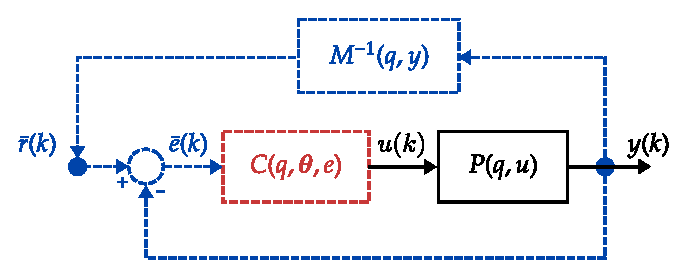
\includegraphics{Figs/diagrama_VRFT.eps}
   \caption{ Experiment to obtain the data used to identify the controller parameters by the VRFT method:
   real data (\textit{black solid lines}), virtual data (\textit{blue dashed lines}) and the cotroller to tune in (\textit{red dashed block}).}
   \label{fig:Figs-diagrama_VRFT-eps}
\end{figure}

\section{Filtro Caso não Linear}%
\label{sec:filtro_caso_não_linear}

Objetivo do filtro
\begin{equation}
   J_{\mathrm{VRFT}}\left(\theta^{+}\right):=\left\|F\left[C_{\theta}+[\tilde{e}]\right]-F[\tilde{u}]\right\|^{2}
   \label{eq:JVR}
\end{equation}
Deseja-se selecionar um filtro tal que \begin{equation}
   \left.\frac{\partial^{2} J_{\mathrm{VRFT}}\left(\theta^{+}\right)}{\partial \theta^{+2}}\right|_{\theta_{0}^{+}}=\left.\frac{\partial^{2} J\left(\theta^{+}\right)}{\partial \theta^{+2}}\right|_{\theta_{0}^{+}}
   \label{eq:condToF}
\end{equation}

\begin{theorem}
   Se 
   \begin{equation}
       F=(I-M D)\left(\left.\frac{\partial P[u]}{\partial u}\right|_{\tilde{u}}\right)
       \label{eq:FiltroVRFTNL}
   \end{equation}
   então \eqref{eq:condToF} é satisfeita.
\end{theorem}


\section{Prova da escolha do filtro VRFT}%
\label{sec:prova_da_escolha_do_filtro_vrft}
Note que
\begin{equation}
\tilde{u}=C_{\theta_{0}^{+}}[\tilde{e}]
\label{eq:uTil}
\end{equation}
uma vez que
\begin{align}
   \tilde{u}&=P^{-1}[\hat{y}]=P^{-1}\left[(I-M D)^{-1}(I-M D) \hat{y}\right] \nonumber\\
            &= P^{-1}\left[(I-M D)^{-1}(M \tilde{r}-M D \tilde{y})\right]=P^{-1}\left[(I-M D)^{-1} M \tilde{e}\right] = C^{0}[\tilde{e}] \nonumber\\
            &=C_{\theta_{0}^{+}}[\tilde{e}].
\end{align}

De forma semelhante
\begin{equation}
   \tilde{y}=y_{\theta_{0}^{+}}
\label{eq:yqp}
\end{equation}
uma vez que, $\tilde{y}=P[\tilde{u}]$ a partir de \eqref{eq:uTil}, assumindo $\tilde{e}=\tilde{r}-D \tilde{y}$,  tem-se que $\tilde{y}=P\left[C_{\theta_{0}^{+}}[\tilde{e}]\right]=$$P\left[C_{\theta_{0}^{+}}[\tilde{r}-D \tilde{y}]\right]$. Como
$y_{\theta_{0}^{+}}=P\left[C_{\theta_{0}^{+}}\left[\tilde{\tilde{r}}-D y_{\theta_{0}^{+}}\right]\right]$, 
$\tilde{y}$ e $y_{\theta_{0}^{+}}$ corresponde ao mesmo $\tilde{r}$ no mapa $r \mapsto y$ dado por $y=P\left[C_{\theta_{0}^{+}}[r-D y]\right]$.
% $\tilde{y}$ e $y_{\theta_{0}^{+}}$ corresponde ao mesmo $\tilde{r}$ in the $r$ to $y$ map given by $y=P\left[C_{\theta_{0}^{+}}[r-D y]\right]$
Uma vez que tal mapa, dado um $r$ há somente um $y$ correspondente, conclui-se \eqref{eq:yqp}.
De \eqref{eq:yqp} é possível concluir que 
\begin{equation}
   \tilde{r}-D y_{\theta_{0}^{+}}=\tilde{e},
\label{eq:eTil}
\end{equation}
que, em \eqref{eq:uTil}, resulta em
\begin{equation}
\tilde{u}=C_{\theta_{0}^{+}}\left[\tilde{r}-D y_{\theta_{0}^{+}}\right].
\label{eq:uTil_2}
\end{equation}

% Parei aqui...

Por simplicidade e maior clareza no desenvolvimento, adota-se a seguinte notação:
\begin{align}
   x_{\theta^{+}} &\triangleq F\left[C_{\theta^{+}}[\tilde{e}]\right]-F[\tilde{u}] \label{eq:x} \\
   w_{\theta^{+}} &\triangleq y_{\theta^{+}}-\tilde{y} \label{eq:w} \\
   \frac{\partial g}{\partial \theta^{+}} &\triangleq 
   \begin{bmatrix} 
      \partial g_1/\partial \theta^{+}_1 & \dots & \partial g_1/\partial \theta^{+}_j & \dots & \partial g_1/\partial \theta^{+}_{n_{\theta +}} \\
      \vdots &  & \vdots & & \vdots \\
      \partial g_i/\partial \theta^{+}_1 & \dots & \partial g_i/\partial \theta^{+}_j & \dots & \partial g_i/\partial \theta^{+}_{n_{\theta +}} \\
      \vdots & & \vdots & & \vdots \\
      \partial g_N/\partial \theta^{+}_1 & \dots & \partial g_N/\partial \theta^{+}_j & \dots & \partial g_N/\partial \theta^{+}_{n_{\theta +}}
   \end{bmatrix} \label{eq:partg}
\end{align}
   % \partial g /\partial \theta^{+} &\triangleq \partial g(i)  /\partial \theta^{+}_j \label{eq:partg}
\todo{Olhar \eqref{eq:partg}. Não é bem isso, na verdade é uma matriz.} 
Sendo \eqref{eq:partg} (em que $g$ é uma função genérica) definida tal que o $(i,j)$-ésimo elemento é $\partial g(i)  /\partial \theta^{+}_j$, de modo que as colunas $(j)$ correspondem às derivadas de $g$ em relação a diferentes parâmetros e as linhas $(i)$ correspondem à evolução temporal.

Usando \eqref{eq:x} e \eqref{eq:w}, as função de custo \eqref{eq:JVR} e \eqref{eq:Jy} são rescritas como
$$
J_{\mathrm{VR}}\left(\theta^{+}\right)=\left\|x_{\theta^{+}}\right\|^{2} \qquad J\left(\theta^{+}\right)=\left\|w_{\theta^{+}}\right\|^{2}
$$
Calculando a primeira e segunda derivadas de $J_{\mathrm{VR}}\left(\theta^{+}\right)$ com respeito ao vetor de parâmetros $\theta^+$, para aproximação por séries de Taylor:
\begin{align}
   \frac{\partial J_{\mathrm{VR}}\left(\theta^{+}\right)}{\partial \theta^{+}} &=\frac{\partial x_{\theta^{+}}^{T} x_{\theta^{+}}}{\partial \theta^{+}} = 2 x_{\theta^{+}}^{T}\left(\frac{\partial x_{\theta^{+}}}{\partial \theta^{+}}\right), \\
\frac{\partial^{2} J_{\mathrm{VR}}\left(\theta^{+}\right)}{\partial \theta^{+2}}&= 2 x_{\theta^{+}}^{T}\left(\frac{\partial^{2} x_{\theta^{+}}}{\partial \theta^{+2}}\right)
+2\left(\frac{\partial x_{\theta^{+}}}{\partial \theta^{+}}\right)^{T}\left(\frac{\partial x_{\theta^{+}}}{\partial \theta^{+}}\right). 
\end{align}
Utilizando \eqref{eq:x} e \eqref{eq:uTil} e calculando as derivadas para o ponto de equilíbrio $\theta^{+}_0$, resulta em
\begin{align}
\left.J_{\mathrm{VR}}\left(\theta^{+}\right)\right|_{\theta_{0}^{+}}
& =\left.\frac{\partial J_{\mathrm{VR}}\left(\theta^{+}\right)}{\partial \theta^{+}}\right|_{\theta_{0}^{+}} =0 \label{eq:JVRTaylor_1}\\
   \left.\frac{\partial^{2} J_{\mathrm{VRFT}}\left(\theta^{+}\right)}{\partial \theta^{+2}}\right|_{\theta_{0}^{+}} &= 2\left(\left.\frac{\partial x_{\theta^{+}}}{\partial \theta^{+}}\right|_{\theta_{0}^{+}}\right)^{T}\left(\left.\frac{\partial x_{\theta^{+}}}{\partial \theta^{+}}\right|_{\theta_{0}^{+}}\right) \label{eq:JVRTaylor_2}
\end{align}

Fazendo o mesmo procedimento para $J\left(\theta^{+}\right)=\left\|w_{\theta^{+}}\right\|^{2}$:
\begin{align}
\frac{\partial J\left(\theta^{+}\right)}{\partial \theta^{+}} 
   &=\frac{\partial w_{\theta^{+}}^{T} w_{\theta^{+}}}{\partial \theta^{+}}=2 w_{\theta^{+}}^{T}\left(\frac{\partial w_{\theta^{+}}}{\partial \theta^{+}}\right), \\
\frac{\partial^{2} J\left(\theta^{+}\right)}{\partial \theta^{+2}}&= 2 x_{\theta^{+}}^{T}\left(\frac{\partial^{2} w_{\theta^{+}}}{\partial \theta^{+2}}\right) 
+2\left(\frac{\partial w_{\theta^{+}}}{\partial \theta^{+}}\right)^{T}\left(\frac{\partial w_{\theta^{+}}}{\partial \theta^{+}}\right).
\label{eq:}
\end{align}
Usando \eqref{eq:w} e \eqref{eq:yqp}:
\begin{align}
\left.J\left(\theta^{+}\right)\right|_{\theta_{0}^{+}}                                                                      
&=\left.\frac{\partial J\left(\theta^{+}\right)}{\partial \theta^{+}}\right|_{\theta_{0}^{+}}=0 \label{eq:JyTaylor_1} \\
   \left.\frac{\partial^{2} J\left(\theta^{+}\right)}{\partial \theta^{+2}}\right|_{\theta_{0}^{+}} &= 2\left(\left.\frac{\partial w_{\theta^{+}}}{\partial \theta^{+}}\right|_{\theta_{0}^{+}}\right)^{T}\left(\left.\frac{\partial w_{\theta^{+}}}{\partial \theta^{+}}\right|_{\theta_{0}^{+}}\right) . \label{eq:JyTaylor_2}
\end{align}

Somando os termos de \eqref{eq:JVRTaylor_1} a \eqref{eq:JVRTaylor_2}, e os \eqref{eq:JyTaylor_1} e \eqref{eq:JyTaylor_2}, tem-se, respectivamente uma aproximação de segunda ordem por séries de Taylor. E para que o objetivo do filtro \eqref{eq:FiltroVRFTNL} seja alcançado, ou seja $ J_{\mathrm{VR}}\left(\theta^{+}\right) \approx J\left(\theta^{+}\right)$, comparando \eqref{eq:JVRTaylor_2} com \eqref{eq:JyTaylor_2}, deve-se ter  
\begin{equation}
   \left.\frac{\partial x_{\theta^{+}}}{\partial \theta^{+}}\right|_{\theta_{0}^{+}}=\left.\frac{\partial w_{\theta^{+}}}{\partial \theta^{+}}\right|_{\theta_{0}^{+}}
   \label{eq:FilterObjective}
\end{equation}

Usando a notação 

\begin{equation}
   \frac{\partial P[u]}{\partial u} \triangleq 
   \begin{bmatrix} 
      \partial P[u]_1/\partial u_0 & \dots & \partial P[u]_1/\partial u_{(j-1)} & \dots & \partial P[u]_1/\partial u_{(N-1)} \\
      \vdots &  & \vdots & & \vdots \\ 
      \partial P[u]_i/\partial u_0 & \dots & \partial P[u]_i/\partial u_{(j-1)} & \dots & \partial P[u]_i/\partial u_{(N-1)} \\
      \vdots & & \vdots & & \vdots \\ 
      \partial P[u]_N/\partial u_0 & \dots & \partial P[u]_N/\partial u_{(j-1)} & \dots & \partial P[u]_N/\partial u_{(N-1)}
   \end{bmatrix}  
   \label{eq:PuDu}
\end{equation}
e resolvendo o lado esquerdo de \eqref{eq:FilterObjective}, considerando que o filtro $F$ é linear, chega-se a
\begin{equation}
   \left.\frac{\partial x_{\theta^{+}}}{\partial \theta^{+}}\right|_{\theta_{0}^{+}}=\left.\frac{\partial F\left[C_{\theta^{+}}[\tilde{e}]\right]}{\partial \theta^{+}}\right|_{\theta_{0}^{+}}=F\left(\left.\frac{\partial C_{\theta^{+}}[\tilde{e}]}{\partial \theta^{+}}\right|_{\theta_{0}^{+}}\right)
\label{eq:28}
\end{equation}

Como $C_{\theta_0^+} = \tilde{u}$, ver \eqref{eq:uTil}, o lado direito de \eqref{eq:FilterObjective} é calculado como
\begin{align}
\left.\left.\frac{\partial P[u]}{\partial u}\right|_{\tilde{u}} \frac{\partial C_{\theta_{0}^{+}}[e]}{\partial e}\right|_{\tilde{e}} &=\left.\frac{\partial P\left[C_{\theta_{0}^{+}}[e]\right]}{\partial e}\right|_{\tilde{e}} \nonumber\\
&=\left.\frac{\partial(I-M D)^{-1} M[e]}{\partial e}\right|_{\tilde{e}} \nonumber\\
&=(I-M D)^{-1} M .
\label{eq:29}
\end{align}

Aplicando a regra da cadeia, em $(\partial y_{\theta_0^+}/\partial \theta^+)$:
\begin{align}
\left.\frac{\partial y_{\theta^{+}}}{\partial \theta^{+}}\right|_{\theta_{0}^{+}}=&\left.\frac{\partial P\left[C_{\theta^{+}}\left[\tilde{r}-D y_{\theta^{+}}\right]\right]}{\partial \theta^{+}}\right|_{\theta_{0}^{+}} \\
=&\left.\frac{\partial P[u]}{\partial u}\right|_{C_{\theta_{0}^{+}}\left[\tilde{r}-D y_{\theta_{0}^{+}}\right]} 
   \left\{\left.\left.\frac{\partial C_{\theta^{+}}\left[\tilde{r}-D y_{\theta_{0}^{+}}\right]}{\partial \theta^{+}}\right|_{\theta_{0}^{+}}{-\left.\frac{\partial C_{\theta_{0}^{+}}[e]}{\partial e}\right|_{\tilde{r}-D y_{\theta_{0}^{+}}}} \frac{\partial D y_{\theta^{+}}}{\partial \theta^{+}}\right|_{\theta_{0}^{+}}\right\}
\end{align}
%
Usando \eqref{eq:eTil} e \eqref{eq:uTil_2},
\begin{equation}
   \left.\frac{\partial y_{\theta^{+}}}{\partial \theta^{+}}\right|_{\theta_{0}^{+}}=\left.\frac{\partial P[u]}{\partial u}\right|_{\tilde{u}}\left\{\left.\frac{\partial C_{\theta^{+}}[\tilde{e}]}{\partial \theta^{+}}\right|_{\theta_{0}^{+}}\right.
   \left.-\left.\left.\frac{\partial C_{\theta_{0}^{+}}[e]}{\partial e}\right|_{\tilde{e}} \frac{\partial D y_{\theta^{+}}}{\partial \theta^{+}}\right|_{\theta_{0}^{+}}\right\}
\end{equation}


e então
\begin{equation}
   \left.\left.\frac{\partial P[u]}{\partial u}\right|_{\tilde{u}} \frac{\partial C_{\theta^{+}}[\tilde{e}]}{\partial \theta^{+}}\right|_{\theta_{0}^{+}}
   =
   \left.\frac{\partial y_{\theta^{+}}}{\partial \theta^{+}}\right|_{\theta_{0}^{+}}+\left.\left.\left.\frac{\partial P[u]}{\partial u}\right|_{\tilde{u}} \frac{\partial C_{\theta_{0}^{+}}[e]}{\partial e}\right|_{\tilde{e}} \frac{\partial D y_{\theta^{+}}}{\partial \theta^{+}}\right|_{\theta_{0}^{+}}.
\end{equation}

Substituindo em \eqref{eq:29} resulta em
\begin{equation}
   \left.\frac{\partial y_{\theta^{+}}}{\partial \theta^{+}}\right|_{\theta_{0}^{+}}+(I-M D)^{-1} M \frac{\partial D y_{\theta^{+}}}{\partial \theta^{+}} \left.\right|_{\theta_{0}^{+}}
   =\left.\left.\frac{\partial P[u]}{\partial u}\right|_{\tilde{u}} \frac{\partial C_{\theta^{+}}[\tilde{e}]}{\partial \theta^{+}}\right|_{\theta_{0}^{+}},
\end{equation}
que, multiplicando por $(I-MD)$, nos dá
\begin{equation}
   \left.\frac{\partial y_{\theta^{+}}}{\partial \theta^{+}}\right|_{\theta_{0}^{+}}-\left.M D \frac{\partial y_{\theta^{+}}}{\partial \theta^{+}}\right|_{\theta_{0}^{+}}+\left.M \frac{\partial D y_{\theta^{+}}}{\partial \theta^{+}}\right|_{\theta_{0}^{+}}
   =\left.\left.(I-M D) \frac{\partial P[u]}{\partial u}\right|_{\tilde{u}} \frac{\partial C_{\theta^{+}}[\tilde{e}]}{\partial \theta^{+}}\right|_{\theta_{0}^{+}}
\end{equation}
Por fim, o termo do lado direito de \eqref{eq:FilterObjective}, pode ser escrito como
\begin{equation}
   \left.\frac{\partial w_{\theta^{+}}}{\partial \theta^{+}}\right|_{\theta_{0}^{+}} =\left.\frac{\partial y_{\theta^{+}}}{\partial \theta^{+}}\right|_{\theta_{0}^{+}} 
   =\left.\left.(I-M D) \frac{\partial P[u]}{\partial u}\right|_{\tilde{u}} \frac{\partial C_{\theta^{+}}[\tilde{e}]}{\partial \theta^{+}}\right|_{\theta_{0}^{+}}
\end{equation}
que, comparando com \eqref{eq:28}, conclui-se que
\begin{equation}
   F=(I-M D)\left(\left.\frac{\partial P[u]}{\partial u}\right|_{\tilde{u}}\right) .
\label{eq:FiltroFinal}
\end{equation}



 \clearpage
 \thispagestyle{empty}
 \cleardoublepage
% % }}} ------------------------------------------------------------------

% {{{ Captulo 4 - Reinforcement Learning

% -*- TeX-master: "Qualificacao.tex" -*-
%!TEX root = Qualificacao.tex
\chapter{Reinforcement Learning}\label{cap:RL}
\vspace{-1cm}

% Frase citação inicial {{{1
% \begin{flushright}
% \begin{minipage}{0.7\linewidth}
%     \emph{``\dots''}
% \end{minipage}
% \end{flushright}
%
% \begin{flushright}
% Cicrano
% \end{flushright}
%
%\vspace{1cm}

O Capítulo de RL vai aqui.


% \input{chapter4_RL.tex}
  \clearpage
  \thispagestyle{empty}
  \cleardoublepage
% % }}} ------------------------------------------------------------------

% {{{ Capitulo 5 - Resultados Simulados
%!TEX root = Qualificacao.tex

\chapter{Randomized Controller Structure Selection}\label{cap:CCS}
\vspace{-1cm}

% Frase citação inicial {{{1
% \begin{flushright}
% \begin{minipage}{0.7\linewidth}
%     \emph{``\dots''}
% \end{minipage}
% \end{flushright}
%
% \begin{flushright}
% Cicrano
% \end{flushright}
%
%\vspace{1cm}

% Intro CAP {{{2

In this chapter, proposals for the design of DDC controllers, with regard to the choice of controller structure are presented. The methodology used, as well as the preliminary results obtained in a first stages of this research are presented.

In this research, focus has been given to the study and development of structure selection techniques for the model of feedback controllers in a DDC\@ design fashion.
The intention is, at first, in the scope of non-linear control systems, to adapt known techniques of structure selection in the area of systems identification to deal with the control case, where the system to be identified becomes the controller. To achieve these objectives, it was decided, to use polynomial models to represent the controllers, initially with NARX structures. This choice is convenient due to the structural flexibility characteristic and the ability of these models to describe non-linear systems~\citep{pearson1999, martins2013}.
% \begin{figure}[htpb]
% \centering
% \missingfigure{Pretendo colocar por aqui um diagramas (deve ser blocos) para ajudar.}
% % \includegraphics[width=0.8\textwidth]{}
% \caption{}
% \label{fig:Diagrama representativo}
% \end{figure}
%

As mentioned in Chapter~\ref{cap:cap2}, one of the main steps in the system identification procedure from data is the step of choosing the model structure. Works that aim to help on this task have been proposed, as is the case of the papers published  by~\cite{baldacchino2012,baldacchino2013} and \cite{falsone2014,falsone2015},
\todo{Vou colocar aqui mais referências neste sentido, de seleção de estruturas} 
in which a random approach is used in order to select the best candidates among the possible regressors in the formation of the model to be identified.

% As mentioned in Chapter~\ref{cap:cap2}, one of the main steps in the procedure of model system identification from data is the model selection step.  Studies that aim to deal with this task have been proposed, as is the case of studies developed by~\cite{falsone2014, falsone2015} in which a random approach, named RaMSS, is used in order to select the best candidates to compose a final model structure, among a class of possible regressors.
%
% \todo{Confirmar se o RaMSS original só é aplicável a NARX mesmo na sua forma original. Se for, falar aqui.}
More recently, ~\cite{retesNARMAXModelIdentification2019} extended the RaMSS strategy for choosing NARMAX model structures, which take into account the effect of noise on signals in order to reduce the polarization in parametric estimates.

In the scope of controller design based on data, more specifically by the VRFT method, in which the controller parameters are adjusted by conventional identification techniques such as OLS, ILS, IV, among others, the same problem of choosing the model structure occurs, with the difference that the model now represents the controller, and no longer the process. Therefore, analogies must be able to be made intended to use the RaMSS method in order to extend it for the purpose of identifying the most suitable structure for the controller.

In this sense, the present work has been directed to the study of the possibilities and consequences of using these technologies for control purposes, aiming to choose the most suitable controller structure.

\todo[inline]{Pretendo colocar um paragrafo aqui comentando o que será apresentado no restante do capítulo.} 


\section{Methodology}\label{sec:CSS_metod} \todo{Talvez colocar o Título como: ``The RaCSS Methodology''"?}
\todo[inline]{A terminar... Vou mexer no início e fim desta seção ainda, enquanto estiver traduzindo.} 

% Como metodologia para atingir este objetivo, listam-se as etapas a seguir, que por sua vez são detalhadas nas seções subsequentes:
Visando atingir o objetivo final de se utilizar uma estratégia para estrutura e identificação paramétrica de controladores a partir de uma abordagem DDC, pretende-se neste trabalho, fazer uso das duas metodologias abordadas em capítulos anteriores: o VRFT, para sintonia de parâmetros do controlador e o RaMSS, para seleção da melhor estrutura do controlador. A partir de do estudo e adaptações de trabalhos anteriores \citep{retesNARMAXModelIdentification2019}, tem-se desenvolvido um algoritmo capaz de unir as duas estratégias com o objetivo de auxiliar tanto na seleção de estruturas, quando na sintodia de controladores não-lieares (ou lineares). O algoritmo tem servido de  framework para estudo e validação da abordagem proposta, a partir de simuações numéricas. Neste sentido, parte dos esforços da pesquisa tem se voltado para a implemetação numérica deste framework. Em uma primeira etapa, foi analisado o comportamento do algoritmo na identificação de modelos de processos, a partir do algoritmo RaMSS, como proposto originalmente. Alguns dos resultados de validação desta etapa são apresentados no Capítulo \ref{cap:cap2}, sob a forma do Exemplo \ref{ex:varHeater}.

Uma vez validado o funcionamento do algorítmo, o método VRFT, discutido no Capítulo \ref{cap:VRFT} é acrescentado ao processo, de forma que o desempenho do RaMSS em selecionar estruturas para um controlador possa ser avaliado na prática.
Nesta etapa, o algoritmo RamSS, utilizado no Capítulo \ref{cap:cap2} é ligeiramente modificado para lidar com a esimação paramétrica via VRFT, para primeiros testes de projeto de controladores. Neste cenário se espera alguns primeiros resultados, sem maiores compromissos com bons desempenhos, mas de são de grande valia para análise e comparação das modificações propostas. Alguns destes resuldados são apresentados pelos exemplos da seção \ref{sec:prel_results} a seguir, mais especificamente no exemplo \ref{ex:51}.

Como abordado no Capítulo \ref{cap:VRFT}, sob certas condições, o controlador pode ser identificados por procedimentos tradicionais de identificação de sistemas pelo método VRFT. Caso as condições necessárias não sejam satisfeitas (vide a Assumption \ref{ass:machedControl} -- matched control) um filtro pode ser projetado de forma que a minimização do índice de custo relativo aos sinais de entrada e saída do controlador, dado por $J_{VR}(\bm{\theta})$ resulte também na minimização do índice de custo $J_{MR}(\bm{\theta})$ relativo ao erro de rastreamento de um modelo de referência. Esta relação é garantida pelo filtro desde que a estrutura do modelo não seja muito ``distante'' da estrutura ideal, i.e. desde que não seja muito subparametrizada.

Uma proposta é utilizar o procedimento RaMSS para tentar identificar a estrutura ideal para o controlador, ou pelo menos uma estrutura próxima que gere bons resultados ao se utilizar o procedimento VRFT. A identificação desta estrutura é feita a partir de dados colhidos sob a abordagem VRFT. Na tentativa de validar a proposta simulações são feitas em diferentes cenários. 
Em um primeiro cenário o procedimento RaMSS é aplicado a um processo linear onde seu modelo e o modelo do controlador ideal são previamente conhecidos. O intuito aqui é analisar o comportamento do procedimento na seleção de regressores candidatos a um eventual controlador. Uma análise ao estilo Monte Carlo é aplicada ao processo em 2 casos: no primeiro, o procedimento é realizado sem influência de ruídos nos dados utilizados; no segundo, ruídos são acrescentados aos dados no intuito de simulação de um ambiente mais realista. O Exemplo \ref{ex:sis2aord} analisa estes casos.

O procedimento RaMSS foi originalmente proposto para lidar com identificação de processos, e não controladores.
A atualização do vetor de probabilidades para inclusão dos regressores (RIPs) é feita baseando-se em índices de desempenho visando avaliar a qualidade de predição do modelo. 
Esta predição é feita sobre dados de treinamento, utilizando uma versão exponencial do MSSE, e possivelmente, no intuito de aumentar a robustez, sobre dados de validação (free run simulation) por meio de uma versão exponencial do MSSE.
No entanto, para fins de controle, tais índices podem não ser os melhores.
Principalmente o índice baseado no MSSE, que exige maior custo computacional sob a proposta de promover melhoras na robustez do modelo identificado. O efeito é uma melhor predição do sinal de saída do do modelo identificado, mesmo quando excitado com sinais diferentes daqueles usados na identificação. 
Apesar de carecer de mais estudos, a princípio este índice não parece trazer muitos benefícios quando utilizado para fins MSS do controlador, uma vez que o intuito final, no projeto de um controlador, é fazer com que o sinal de saída do processo (e não do controlador), tenha um comportamento desejado. 

Neste sentido, propõe-se adaptações ao método RaMSS original visando objetivos mais adequados a MSS de controladores. Uma modificação estudada, é a substituição da versão exponencial do MSSE, dada por $J_s= e^{-K\cdot MSSE}$, por uma que leve em conta o rastreamento do sistema em malha fechada, um dos principais objetivos do controlador. Este novo índice é definido como
\begin{equation}
  J_r=e^{-K\cdot MSTE},
  \label{eq:}
\end{equation}
onde $MSTE$, é o erro médio quadrático de rastreamento, definido como 
\begin{equation}
  MSTE = \frac{1}{N}\sum_{k=1}^{N} (y_{rm}(k)-y(k))^2.
  \label{eq:}
\end{equation}

Uma vez que a escolha de estrutura é feita pelo método RaMSS modificado, incorporando elementos da estratégia VRFT, e que o intutito é a seleção de estrutura e parâmetros para controladores, batiza-se, aqui, esta estratégia de \textit{Randomized Controler Structure Selection}, ou RaCSS.

Resultados preliminares do uso deste índice são apresentados nesta qualificação. Os Exemplos \ref{ex:52} e \ref{ex:53} apresentam alguns destes resultados e uma análise geral é feita no Capítulo \ref{cap:Concl}. \todo{colocar a referencia correta aqui.} 

Ressalta-se que os resultados apresentados são preliminares e conclusões concretas ainda não puderam ser apresentadas. 
\todo{batizar o método de RaCSS.} 
No Capítulo \ref{cap:Concl}, propostas para continuidade do trabalho, como inclusão de informações auxiliares ao procedimento, objetivando incorporar características previamente desejadas ou conhecidas para o controlador, assim como possivelmente o uso de estratégias de aprendizado por reforço, no intuito de reduzir o custo computacional devido ao uso de informações da malha fechada do controlador são apresentadas.

Por fim, discussões a respeito de estabilidade, convergência, polarização e robustez são apresentadas, ainda não em um contexto de garantias, mas como conjecturas de passos que pretende-se aprofundar na sequência da presente pesquisa.

\section{Preliminary Results}\label{sec:prel_results}

\begin{exmp}[Second order Linear System -- continued.]\label{ex:sis2aord}

  Consider the 2nd-order linear system describe in Example \ref{exm:31}: 
  \begin{equation}
    \label{eq:sis2aord}
    y_k = a_1y_{k-1} + a_2y_{k-2} + b_1u_{k-1} + b_2u_{k-2}.
  \end{equation}
  % onde, para $i = 1,\ 2$, os termos $a_i$, $b_i$ $\in \R$, representam parâmetros constantes; $u_{k-i}$ e $y_{k-i}$ $\in \R$, os sinais de entrada e saída, respectivamente; e $k$ o índice temporal.
  According to the VRFT strategy (Chapter ~\ref{cap:VRFT}), one must first define a class of allowable controllers $\mathscr{C}$, containing the desired controller structure, and define a reference model that expresses the desired close loop system's behavior.

  In this example, we want to analyze the use of the RAmSS algorithm directly, without modifications, in order to find the best structure for a controller designed from the VRFT strategy.
  In order to examine the behavior of the RaMSS Algorithm in finding the best set of regressors, we proceed as follows.

  A feasible reference model is defined, that is, with a relative degree equal to or greater than that of the process. For simplicity, a 1st order model with the same relative degree of the process is chosen, as Example \ref{exm:31}, given by the transfer function
  \begin{equation}
    T_d(z) = \frac{1-A}{z-A},
    \label{eq:mr_sis2aord}
  \end{equation}
  The parameter adopted here is the same as Exemple \ref{exm:31}, i.e. $A = -T_s/\tau_d = 0.8187$. 
  The ideal controller, represented by an ARX model, will be given by the structure composed of the regressors presented in \eqref{eq:exp31_uk}, represented here by
  \begin{equation}
    \label{eq:exp51_contIdeal}
    u_k = \theta_0e_{k} + \theta_1e_{k-1} + \theta_2e_{k-2} + \theta_3u_{k-1} + \theta_4u_{k-2},
  \end{equation}
  and will have the parameters shown in \eqref{eq:exp31_ideal_parameters}, described here as
  \begin{equation}
    \vtheta^\star= \begin{bmatrix} \theta^\star_0 & \theta^\star_1 & \theta^\star_2 & \theta^\star_3 & \theta^\star_4 \end{bmatrix}^T =  \begin{bmatrix} 0.181 & 0.308 &  0.145 &  0.19 & 0.81 \end{bmatrix}^T.
  \label{eq:ex51_ideal_parameters}
\end{equation}
Using the RaMSS algorithm, as discussed in the section ~\ref{sec:ramss}, the procedure is performed for 2 cases:
\begin{description}
  \item[case A] the universe set $\mathscr{M}$ is taken as all possible 3rd degree non linear models formed by the monomials up to 4 delays for input $\tilde{e}_k$ (virtual error) and output $\tilde{u}_k$ (virtual process input) collected data. No noise is considered in this case.
  \item[case B] the same case as case A, but now with a noise given by a gaussian distribution, i.e. $\nu \sim \mathcal{N}(\mu,\sigma)$, where $\mu=0$ is the mean, and $\sigma= 0.1$ is the standard deviation.
\end{description}
The simulation parameters for the 2 cases are shown in the table ~\ref{tab:exp51_param}.


\begin{table}[htpb]
  \centering
  \caption{Parameters for simulating the RaMSS algorithm of the example ~\ref{ex:sis2aord}}\label{tab:exp51_param}
  \begin{tabular}{c|c|c|c|c|c|c|c}
    Caso & $o$ & $n_e$ & $n_m$ & $N_p$ & $N_i$ & $K_J$ & $\gamma$ \\
    \hline
    1 & $ 1 $ & $7$ & $4$ & $100$ & $100$ & $1$ & $0.1$ \\
    2 & $ 2 $ & $7$ & $4$ & $100$ & $100$ & $1$ & $0.1$
  \end{tabular}
\end{table}
\todo[inline]{MEXER NESTA TABELA AINDA! Valores estão errados. Já os modifiquei. Definir parâmetros, etc. Colocar os mais essenciais por aqui e os menos, no appendice. }

Em uma primeira análise o procedimento RaMSS é aplicado a um conjunto de dados de 700 amostras, obtido via procedimento VRFT, em que o filtro do VRFT é considerado unitário, i.e os dados não são filtrados. O mesmo conjunto de dados é aplicado para os 2 casos. A cada iteração escolhe-se aleatoriamente, por uma processo de Bernoulli, 100 modelos candidatos a serem analisados. 

Applying the procedure in both cases, the following controllers are obtained, for a specific realization:
\begin{align*}
  u_1(k) &= 0.193{u}_1(k-1) + 0.805{u}_1(k-2) + 0.001{u}_1(k-3) \\
         &+ 0.181{e}_1(k) + 0.307{e}_1(k-1) + 0.1441 \\
  u_(k) &= 0.751{u}_2(k-1) + 0.241{u}_2(k-2) -0.33{u}_2(k-3) + 0.322{u}_2(k-4) \\
         &+ 0.174{e}_2(k) + 0.197{e}_2(k-1) + 0.048{e}_2(k-2) + 0.049{e}_2(k-3) + 0.0591
  % \label{eq:contEstsis2aord}
\end{align*}
where the index subscribed to the variables represent the respective cases.
The evolution of RIPs during a typical execution is shown in \ref{fig:ex51_RIPevol_2cases}.
\begin{figure}[H]
  \centering
  \includegraphics[width=\textwidth]{Figs/Cap5/ex51_rips_evol_2cases.tex.pdf}
  \caption{Typical evolution of RIPs for choosing regressors for case 1 and 2.}
  \label{fig:ex51_RIPevol_2cases}
\end{figure}


A figura~\ref{fig:Figs-RespostaSist2aordNARX-png} mostra a resposta temporal para os 2 casos.

\begin{figure}[H]
  \sbox0{\blackdottedline} \sbox1{\bluesolidline} \sbox2{\reddashedline} \sbox3{\blackdashdotline} 
  \centering
  \includegraphics[width=1\textwidth]{./Figs/Cap5/ex51_resp_temporal_mf_editado.tex.pdf}
  % \include{./Figs/Cap5/ex51_resp_temporal_mf.tex}
  \caption{Resposta do sistema em malha fechada (gráfico superior) e respectivos erros absolutos (gráfico inferior) utilizando os controladores identificados no caso A (\usebox1) e no caso B (\usebox2). Os sinais de referência (\usebox3) e de reposta do modelo de de referência (\usebox0) são mostrados no gráfico superior.}
  \label{fig:Figs-RespostaSist2aordNARX-png}
\end{figure}

\todo[inline]{Ainda em construção, por enquanto só coloquei alguns dos gráficos que irei utilizar. Comparações, com tabelas comparando resultados do RaCSS com o ERR também serão ainda colocados. Logicamente, com devidas análises.}

\end{exmp}

\begin{exmp}[RaCSS aplicado a um sistema linear de 2$^a$ ordem] \label{ex:52}

  \todo[inline]{    
    Neste exemplo aplico o ``RaCSS'' ao mesmo sistema de 2a ordem do exemplo anterior, mas agora usando informação do erro de rastreamento no cálculo dos RIPs.

    Por enquanto estão somente os gráficos, ainda falta análise e algumas tabelas comparativas com ERR.
  }

  Evolução dos RIPs para um caso típico:

  \begin{figure}[H]
    \centering
    \includegraphics{Figs/Cap5/ex51_rips_evol_SR.tex.pdf}
    \caption{Evolução dos RIPs para diferentes valores da parâmetro $\alpha$ considerando dados sem ruído. ({\color{red} Caption ainda será mudada.})}
    \label{fig:exp51_ev_rips_a1}
  \end{figure}

  \begin{figure}[H]
    \centering
    \includegraphics{Figs/Cap5/ex51_rips_evol_CR.tex.pdf}
    \caption{Evolução dos RIPs para diferentes valores da parâmetro $\alpha$ considerando dados COM ruído. ({\color{red} Caption ainda será mudada.})}
    \label{fig:exp51_ev_rips_a1}
  \end{figure}



  Convergência dos regressores para 100 simulações para cada parâmetro $\alpha$ diferente:

  \begin{figure}[H]
    \centering
    \includegraphics{Figs/Cap5/ex51_iter_con_SEM_ruido.tex.pdf}
    \caption{Densidades de probabilidades para os regressores escolhidos para diferentes valores de $\alpha$, caso sem ruído.({\color{red} Caption ainda será mudada.})}
    \label{fig:exp51_itercon_ruido}
  \end{figure}

  \begin{figure}[H]
    \centering
    \includegraphics{Figs/Cap5/ex51_iter_con_COM_ruido.tex.pdf}
    \caption{Densidades de probabilidades para os regressores escolhidos para diferentes valores de $\alpha$, caso COM ruído.({\color{red} Caption ainda será mudada.})}
    \label{fig:exp51_itercon_ruido}
  \end{figure}



\end{exmp}


\begin{exmp}[RaCSS aplicado a um sistema não-linear] \label{ex:53}

  \todo[inline]{
    Neste exemplo a ideia é avaliar o comportamento do ``RaCSS'' a um sistema não-linear. Tomei um modelo de um aquecedor com dissipação variável adotado no seu livro. A ideia é apresentado o modelo no exemplo~\ref{ex:varHeater} da seção~\ref{sec:ramss}, no sentido do RaMSS para identificar o modelo. Depois aproveito o mesmo aqui para identificar o controlador.

    Por enquanto estão somente os gráficos, ainda falta análise e algumas tabelas comparativas com ERR.
  }



\end{exmp}
% =================================================================================================================

% \newpage
% \section{Rascunho}\label{sec:Rascunho}
%
%
% Como produto/trabalho em desenvolvimento durante o semestre, cita-se o trabalho que tem sido feito no sentido de desenvolver metodologias para escolha de estruturas para o controlador no âmbito do controle baseado em dados, ou DDC (Data-Driven Control).
% Mais especificamente, tem-se dado ênfase a escolha da estrutura do controlador a partir do uso de métodos VRFT.
% Como deixa claro em seu nome, ao usar o termo “sintonia” (em inglês, “tunning” ), a metodologia VR  FT visa a sintonia de um controlador pertencente a uma classe de controladores pré-estabelecida.
% Como abordado pelos autores do método~\citep{campi2002,campi2006a}, por outros estudiosos do assunto~\citep{bazanella2012} e apresentado neste relatório na seção de revisão bibliográfica, o método visa minimizar o erro de rastreamento de um modelo de referência pré-definido a partir da minimização de uma função de custo.
% Tal função é definida a partir do erro quadrático entre o sinal de excitação utilizado no processo a se controlar e o sinal de controle “virtual”, gerado pelo controlador identificado ao se aplicar  o mesmo sinal de referência capaz de produzir o mesmo sinal de saída  virtual utilizado na identificação.
%~\cite{campi2002} mostram, para o caso linear, e~\cite{campi2006}  e não linear, que ao se minimizar esta nova função de custos, minimiza-se também o erro de rastreamento, desde que se obedeça os seguintes critérios: a classe do controlador considerado tenha uma estrutura que possibilite abrigar o que se nomeia de controlador ideal (vide eq.
% ); que o processo não seja afetado por ruídos; e o controlador seja parametrizado linearmente.
% Caso o controlador ideal não possa ser representado pela classe considerada, o erro mínimo de rastreamento não é mais garantido e a introdução de um filtro ao projeto, visando se aproximar desse mínimo é desejado.
%
%
% No desenvolvimento do trabalho, foco deste relatório, tem-se feito um estudo de como seria possível, e quais as vantagens poderia-se obter se, ao invés de apenas tentar achar a melhor sintonia para um controlador com estrutura pré-estabelecida,  se procurasse também uma melhor estrutura dentro de um um conjunto de classes de controladores, de forma que o erro de rastreamento ótimo ou pelo menos sub-ótimo possa ser encontrado.
%
% Para atingir este propósito, tem-se investigado o uso de técnicas de seleção de estruturas que, com devidas adaptações e reformulações, sejam capazes selecionar modelos que resultem em controladores não lineares (ou mesmo lineares) que possam levar a respostas melhores do que aqueles que fazem uso de estruturas pré definidas.
%
% Dentre as ferramentas que têm-se utilizado, destacam-se o uso da taxa de redução de erro (ERR) e do algoritmo   Randomized Model Structure Selection (RaMSS)~\citep{falsone2014,falsone2015}. Estas estratégias têm sido estendidas e utilizadas em aplicações para determinação de modelos de processos dinâmicos~\citep{retesNARMAXModelIdentification2019} ou até mesmo no projeto de compensadores para aplicações em que o processo exibe determinados efeitos de não linearidade específicas, como no caso de efeitos histeréticos~\citep{abreuIdentificationNonlinearityCompensation2020}.

% Em particular, o método RaMSS, tem se mostrado promissor para a aplicação desejada. Esse método faz apelo às técnicas exploratórias que recorrem a buscas aleatórias ao estilo Monte Carlo, mas com mecanismos de seleção que reduzem drasticamente o custo computacional, evitando uma busca exaustiva, ao mesmo tempo em que tenta garantir uma seleção adequada.
%
% Apoiado nesta técnica, algumas adaptações têm sido estudadas no sentido de lidar agora com a identificação do controlador, e não mais do processo.
%
% Como abordado na revisão bibliográfica deste relatório, o método RaMSS faz uso de um índice de desempenho baseado no cálculo de alguma grandeza que quantifique a qualidade de o modelo em algum sentido. Uma escolha comum é calcular este índice baseado no erro quadrático médio de predição (MSPE).
%
% Um estudo sobre o uso deste índice tem sido feito na pesquisa em questão, conforme resultados apresentados na seção “Análise e Processamento de Dados”. O que se tem observado é que minimizar o MSPE diretamete pela estratégia RaMSS apesar de muitas vezes apresentar bons resultados, não dá garantias que o rastreamento ótimo é alcançado, i.e. aquele em que o erro de rastreamento médio quadrático por exemplo, é mínimo.
%
% Para sanar  esta deficiência, tem-se considerado o uso de algum índice que leve em conta o resultado final ao se aplicar os controladores intermediários identificados e selecionados pelo procedimento. Algo parecido tem sido usado no que diz respeito a identificação de processos  em que o erro quadrático médio de simulação (MSSE) é utilizado em substituição ao MSPE~\citep{aguirre2010}. Neste caso, segundo~\citep{piroddi2003}, o uso de informações da simulação-livre pode melhorar a robustez na seleção de estrutura do processo quando sob condições de identificabilidade parciais.
%
% O MSSE depende da simulação livre, que em suma é a resposta em malha aberta a um sinal de excitação conhecido. Algo parecido poderia ser utilizado ao se avaliar a estrutura no procedimento VRFT, porém, neste caso, seria desejável a resposta do sistema em malha fechada com o controlador obtido a partir da estrutura avaliada. O grande problema neste caso é que esta simulação passa a ser dependente de um modelo, ainda que aproximado do processo. Porém, como estratégias DDC visam exatamente não identificar um modelo para o processo, tal simulação torna-se inviável.
%
% No atual estágio desta pesquisa, tem-se trabalhado com a ideia de um índice que quantifique o erro médio de rastreamento em função do modelo do controlador sintonizado por uma estratégia VRFT, de modo que alguma informação da resposta em malha fechada com o controlador analisado possa ser usada para  o cálculo dos índices de probabilidades de inclusão do regressor, ou RIP (vide seção de Revisão Bibliográfica). Porém, como a simulação da resposta em malha fechada (ou mesmo malha aberta) é inviável devido a uma falta de modelo para o processo, o que se estuda é o uso de técnicas de Aprendizado por Reforço (RL) para que dados colhidos do processo real, enquanto em funcionamento, possam ser usados para o cálculo em tempo real dos RIP e consequentemente para  escolha de melhor estrutura.
%
% Algumas técnicas de RL se mostram promissoras neste caso, uma vez que muitas vezes levam à otimização de índices de desempenho a partir de dados amostrados, sem a necessidade do modelo do processo, ao mesmo tempo em que evitam o alto número de realizações amostrais como em metodologias Monte Carlo. Dentre elas a estratégia TD Learning, tem sido considerada, com uma atenção ao método conhecido como Q-learning, que permite que um controlador possa ser ajustado em uma abordagem conhecida como off-policy. Nesse caso, um controlador ou lei de controle (no caso do presente trabalho, mais precisamente sua estrutura) pode ser determinado enquanto o sistema em malha fechada obedece a uma lei (ou política) de controle diferente. Isto ajuda em eventuais problemas de instabilidade e exploração.
%
% Durante o semestre tem sido desenvolvido um algoritmo no intuito de implementar as ideiais consideradas anteriormente. Parte do algoritmo desenvolvido por Retes (2018), tem sido aproveitada, assim como algoritmos implementados e desenvolvidos pelo grupo do MACSIN1, grupo do qual o autor faz parte desde o início do doutorado. O algoritmo tem sido desenvolvido na linguagem R, portanto traduções de algumas ferramentas já disponíveis no MACSIN em outras linguagens tiveram e estão tendo que ser adaptadas. Os resultados apresentados na seção “Análise e Processamento de Dados” foram obtidos, em sua maioria, a partir deste algoritmo.


  \clearpage
  \thispagestyle{empty}
  \cleardoublepage
% }}} ------------------------------------------------------------------

% {{{ Capitulo 6 - Conclusoes
  % -*- TeX-master: "Qualificacao.tex" -*-
%!TEX root = Qualificacao.tex

\chapter{Conclusions}\label{cap:Concl}
\vspace{-1cm}

% Frase citação inicial {{{1
% \begin{flushright}
% \begin{minipage}{0.7\linewidth}
%     \emph{``\dots''}
% \end{minipage}
% \end{flushright}
%
% \begin{flushright}
% Cicrano
% \end{flushright}
%
%\vspace{1cm}



\section{Final Considerations}\label{sec:Cons_finais}

% A atual pesquisa se encontra em fase de desenvolvimento, mas com os primeiros resultados já é possível inferir que a abordagem RaCSS funciona, no sentido em que auxilia na seleção de estruturas e projeto de controladores DDC. Mais análises serão feitas a fim de se obter informações a respeito de robustez, desempenho e limitações do método.
The current research is in the development phase, but with the first results it is already possible to infer that the RaCSS approach works, in the sense that it helps in the selection of structures and design of DDC controllers. Further analysis will be carried out in order to obtain information regarding the method's robustness, performance and limitations.

% Durante o desenvolvimento, algumas propostas para investigação foram surgindo, as quais, em sua maioria ainda não puderam ser investigadas. Como este trabalho se encontra ainda em fase de desenvolvimento, tais propostas são apresentadas como propostas de continuidade e são listadas com mais detalhes na seção seguinte.
During the development, some proposals for investigation were emerging, which, for the most part, could not be investigated until now. As this work is still in the development phase, these proposals are presented as continuity proposals and are listed in more detail in the following section.

% Como produto/trabalho em desenvolvimento durante o semestre, cita-se o trabalho que tem sido feito no sentido de desenvolver metodologias para escolha de estruturas para o controlador no âmbito do controle baseado em dados, ou DDC (Data-Driven Control).
% Mais especificamente, tem-se dado ênfase a escolha da estrutura do controlador a partir do uso de métodos VRFT.
% Como deixa claro em seu nome, ao usar o termo “sintonia” (em inglês, “tunning” ), a metodologia VR  FT visa a sintonia de um controlador pertencente a uma classe de controladores pré-estabelecida.
% Como abordado pelos autores do método \citep{campi2002,campi2006a}, por outros estudiosos do assunto \citep{bazanella2012} e apresentado neste relatório na seção de revisão bibliográfica, o método visa minimizar o erro de rastreamento de um modelo de referência pré-definido a partir da minimização de uma função de custo.
% Tal função é definida a partir do erro quadrático entre o sinal de excitação utilizado no processo a se controlar e o sinal de controle “virtual”, gerado pelo controlador identificado ao se aplicar  o mesmo sinal de referência capaz de produzir o mesmo sinal de saída  virtual utilizado na identificação.
% \cite{campi2002} mostram, para o caso linear, e \cite{campi2006}  e não linear, que ao se minimizar esta nova função de custos, minimiza-se também o erro de rastreamento, desde que se obedeça os seguintes critérios: a classe do controlador considerado tenha uma estrutura que possibilite abrigar o que se nomeia de controlador ideal (vide eq.
% ); que o processo não seja afetado por ruídos; e o controlador seja parametrizado linearmente.
% Caso o controlador ideal não possa ser representado pela classe considerada, o erro mínimo de rastreamento não é mais garantido e a introdução de um filtro ao projeto, visando se aproximar desse mínimo é desejado.
%
%
% No desenvolvimento do trabalho, foco deste relatório, tem-se feito um estudo de como seria possível, e quais as vantagens poderia-se obter se, ao invés de apenas tentar achar a melhor sintonia para um controlador com estrutura pré-estabelecida,  se procurasse também uma melhor estrutura dentro de um um conjunto de classes de controladores, de forma que o erro de rastreamento ótimo ou pelo menos sub-ótimo possa ser encontrado.
%
% Para atingir este propósito, tem-se investigado o uso de técnicas de seleção de estruturas que, com devidas adaptações e reformulações, sejam capazes selecionar modelos que resultem em controladores não lineares (ou mesmo lineares) que possam levar a respostas melhores do que aqueles que fazem uso de estruturas pré definidas.
%
% Dentre as ferramentas que têm-se utilizado, destacam-se o uso da taxa de redução de erro (ERR) e do algoritmo   Randomized Model Structure Selection (RaMSS) \citep{falsone2014,falsone2015}. Estas estratégias têm sido estendidas e utilizadas em aplicações para determinação de modelos de processos dinâmicos \citep{retesNARMAXModelIdentification2019} ou até mesmo no projeto de compensadores para aplicações em que o processo exibe determinados efeitos de não linearidade específicas, como no caso de efeitos histeréticos \citep{abreuIdentificationNonlinearityCompensation2020}.


\section{Continuity proposals}\label{sec:Prop_cont}

% Como produto/trabalho em desenvolvimento durante o semestre, cita-se o trabalho que tem sido feito no sentido de desenvolver metodologias para escolha de estruturas para o controlador no âmbito do controle baseado em dados, ou DDC (Data-Driven Control).

% O principal foco desta pesquisa tem sido o estudo e desenvolvimento de metodologias de projeto de controladores DDC, com foco especial na seleção de estruturas do controlador com o uso da técnica VRFT.
The main focus of this research has been the study and development of design methodologies for DDC controllers, with a special attention on the controller structures selection using the VRFT approach.

% Em particular, o método RaMSS, tem se mostrado promissor para a aplicação desejada. Esse método faz apelo às técnicas exploratórias que recorrem a buscas aleatórias ao estilo Monte Carlo, mas com mecanismos de seleção que reduzem drasticamente o custo computacional, evitando uma busca exaustiva, ao mesmo tempo em que tenta garantir uma seleção adequada de modelos.
In particular, the RaMSS method, has shown to be promising for the desired application. This method appeals to exploratory techniques that uses Monte Carlo-style random searches, but with selection mechanisms that dramatically reduce computational cost, avoiding an exhaustive search, while trying to ensure an adequate selection of regressors.
%
% Apoiado nesta técnica, algumas adaptações têm sido estudadas no sentido de lidar com a identificação e seleção de estrutura do controlador e não mais do processo.
Supported by this technique, some adaptations have been studied in order to deal with the identification and structure selection of the controller, and not of the process, as proposed by RaMSS approach.

% Na sequência apresenta-se itens específicos a serem abordados, que podem ser tomados como propostas de continuidade:
Following, specific items to be addressed are presented, which can be taken as proposals for continuity of the current work:


% Uma primeira proposta diz respeito ao estudo do uso de índices de desempenho que melhor representem a realidade do controlador ao se atualizar os termos de RIPs.

\medskip
\textbf{Proposal 1} 

A first proposal concerns the study of the use of performance indices that best represent the reality of the controller when updating the terms of RIPs.
% Como já abordado, originalmente o RAmSS utiliza medidas como o MSPE e MSSE para esta atualização.
As already discussed (Section \ref{sec:ramss}), the RaMSS originally uses measures such as MSPE and MSSE for the RIPs updates.
% Para fins de modelagem  de processos físicos, onde muitas vezes a predição do comportamento entrada-saída é o alvo, tais índices se mostram adequados \cite{falsone2015}.
For modeling of physical processes purposes, where the prediction of input-output behavior is often the target, such indices are adequate \cite{falsone2015}.
%
% Porém, ao se abordar o problema da idendificação do controlador, a redução do erro de predição, seja ele de passo a frente, como no caso do MSPE ou de simulação livre, como no caso do do MSSE,  nao ha garantia de que o erro de rastreamento seja reduzido.. E em geral, é este erro de rastreamento o principal alvo em sistemas de controle.
However, when dealing with the controller identification problem, the minimization of the prediction error, be it a step-ahead error, as in the case of MSPE or a free simulation error, as in the case of MSSE, there is no guarantee that the error of tracking is reduced. And in general, this tracking error is the main target in control systems.
%
% omo abordado na revisão bibliográfica deste relatório, o método RaMSS faz uso de um índice de desempenho baseado no cálculo de alguma grandeza que quantifique a qualidade de o modelo em algum sentido. Uma escolha comum é calcular este índice baseado no erro quadrático médio de predição (MSPE).
%
% Um estudo sobre o uso deste índice está em andamento\todo{conforme resultados apresentados na seção ???}. O que se tem observado é que minimizar o MSPE diretamete pela estratégia RaMSS apesar de muitas vezes apresentar bons resultados\todo{não esquecer de explicar o porque destes resultados mesmo quando minimizando o MSPE, que no caso de controle fica em função dos sinais de controle e não da saída. Creio que dá para explicar isso no contexto do VRFT, em que minimizar este índice implica em minimizar o MSE de rastreamento sob certas condições.}, não dá garantias que o rastreamento ótimo é alcançado, i.e. aquele em que o erro de rastreamento médio quadrático é mínimo.
% Um estudo sobre o uso deste índice está em andamento, conforme resultados apresentados no Capítulo \ref{cap:CCS}. O que se tem observado é que minimizar o MSPE diretamete pela estratégia RaMSS apesar de muitas vezes apresentar bons resultados
% não dá garantias que o rastreamento ótimo é alcançado, i.e. aquele em que o erro de rastreamento médio quadrático é mínimo.
\todo{não esquecer de explicar o porque destes resultados mesmo quando minimizando o MSPE, que no caso de controle fica em função dos sinais de controle e não da saída. Creio que dá para explicar isso no contexto do VRFT, em que minimizar este índice implica em minimizar o MSE de rastreamento sob certas condições.}, 
A study on the use of this index is underway, according to results presented in Chapter \ref{cap:CCS}. What has been observed is that minimizing the MSPE directly by the RaMSS strategy, despite often showing good results at prediction of the controller output view point, does not guarantee that the optimal tracking is achieved, i.e. the one in which the mean squared tracking error is minimal.

% Como alternativa, propõe-se o uso de algum índice que leve em conta o resultado em malha fechada ao se aplicar os controladores intermediários identificados e selecionados pelo procedimento. Algo parecido tem sido usado no que diz respeito a identificação de processos  em que o erro quadrático médio de simulação (MSSE) é utilizado em substituição ao MSPE \citep{aguirre2010}. Neste caso, segundo \citep{piroddi2003}, o uso de informações da simulação-livre pode melhorar a robustez na seleção de estrutura do processo quando sob condições de identificabilidade parciais.
As an alternative, it is proposed to use an index that takes into account the result in closed loop when applying the intermediate controllers identified and selected by the procedure. Something similar has been used with regard to the identification of processes in which the mean quadratic simulation error (MSSE) is used to replace the MSPE \citep{aguirre2010}. In this case, according to \citep {piroddi2003}, the use of information from the free simulation can improve the robustness in the selection of the process structure when under partial identifiability conditions.

% O MSSE depende da simulação livre, que em suma é a resposta em malha aberta a um sinal de excitação conhecido. Algo parecido poderia ser utilizado ao se avaliar a estrutura no procedimento VRFT, porém, neste caso, seria desejável a resposta do sistema em malha fechada com o controlador obtido a partir da estrutura avaliada. O grande problema neste caso é que esta simulação passa a ser dependente de um modelo, ainda que aproximado, do processo, ou do próprio processo. Porém, como estratégias DDC visam exatamente não identificar um modelo para o processo, tal situação pode ser um empecilho prático. Uma proposta de solução para este problema é apresentada mais a frente neste texto.
The MSSE depends on free-run simulation, which in short is the open loop response to a known (and new) excitation signal. Something similar could be used when evaluating the structure in the VRFT procedure. In this case, it would be desirable to use the system closed loop response with the controller obtained from the evaluated structure to calculate a new index. As discussed in Chapter \ref{cap:CCS}, the MSE of the tracking error seems to be a good choice (see equation \ref{eq:MSTE}). The big problem in this case is that this simulation becomes dependent on a model, even if approximate, on the process, or on the process itself. However, as DDC strategies aim at exactly not identifying a model for the process, such a situation can be a practical obstacle. A proposal for a solution to this problem is presented later in this text.

\medskip
\textbf{Proposal 2} 

% Uma segunda proposta, a qual também vem sendo analisada, consiste no uso de informações auxiliares durante o processo de identificação dos parâmetros do controlador.
A second proposal, which has also been analyzed, consists in the use of auxiliary information during the process of identifying the parameters of the controller.
% Apesar de já terem sido desenvolvidas técnicas para incorporar informação auxiliar no processo de identificação, por exemplo via restrições e otimização multiobjetivo \citep{barroso2006}, todas estas restrições dizem respeito à planta.
Although techniques have already been developed to incorporate auxiliary information in the identification process, for example via restrictions and multiobjective optimization \citep{barroso2006}, all these restrictions are related to the plant.
% Neste sentido surgem questões como: de que forma estas técnicas podem ser usadas na abordagem DDC?
In this sense, questions arise such as: how can these techniques be used in the DDC approach?
% Seria possível encontrar um análogo da informação auxiliar, usada em métodos tradicionais, para estratégias DDC, em que não há informação da planta?
Would it be possible to find an analogue of auxiliary information, used in traditional methods, for DDC strategies, in which there is no plant information?
% Poderia esta ser definida, por exemplo, a partir restrições que garantam aspectos relevantes ao controle, como limitações de ganho devido a saturação de atuadores, inserção de integradores no controlador, além de aspectos relativos a robustez? Neste sentido, um procedimento para garantir a presença de integradores no modelo do controlador já vem sendo estudado, mas ainda sem resultados conclusivos.
Could this auxiliar information be defined, for example, from restrictions that guarantee aspects relevant to control, such as gain limitations due to saturation of actuators, insertion of integrators in the controller, in addition to aspects related to robustness? In this sense, a procedure to guarantee the presence of integrators in the controller model has already been studied, but still with no conclusive results.

\medskip
\textbf{Proposal 3} 

% Outra proposta a ser estudada diz respeito ao estudo do uso de filtros no processo de identificação do controlador, como é comum na estratégia VRFT. Na estratégia, quando o controlador ideal, ou compatível, não pertence à classe de controladores considerada, ou seja, a hipótese \ref{ass:machedControl} não é satisfeita, um filtro a ser aplicado ao sinal usado no processo de identificação deve ser projetado a fim de se aproximar de uma solução ótima, conforme apresentado por \cite{campi2002,campi2006} e discutido no Capítulo \ref{cap:VRFT}.
Another proposal to be studied concerns in the use of filters in the process of identifying the controller, as is common in the VRFT strategy. In this strategy, when the ideal or compatible controller does not belong to the class of controllers considered, that is, the hypothesis \ref{ass:machedControl} is not satisfied, a filter to be applied to the signals and regressors used in the identification process must be designed in order to approach an optimal solution, as presented by \cite{campi2002, campi2006} and discussed in Chapter \ref{cap:VRFT}.
% Até agora, os resultados apresentados no Capítulo \ref{cap:CCS} não fizeram uso deste filtro. Este deve ser o próximo passo a ser adotado no procedimento em desenvolvimento.
So far, the results presented in Chapter \ref{cap:CCS} have not made use of this filter. This should be the next step to be taken in the procedure under development.
\todo{terminar este pensamento} 

\medskip
\textbf{Proposal 4}

% Um problema inerente tanto a metodologias de identificação de sistemas quanto ao método VRFT é a polarização de parâmetros que aparecem quando o processo a se identificar (seja ele a planta ou controlador) está sujeito a ruído colorido. É comum o uso de estimadores de variáveis intrumentais (VI) para amenizar os efeitos da polarização na abordagem VRFT. No trabalho em desenvolvimento propõe-se estudar o uso do estimador de mínimos quadrados estendido (ELS) para este fim.
A inherent problem to both, systems identification methodologies, and the VRFT method, is the polarization of parameters that appear when the process to be identified (be it the plant or controller) is subject to colored noise. It is common to use instrumental variable estimators (VI) to mitigate the effects of polarization in the VRFT approach. It is proposed to study the use of the extended least squares estimator (ELS) during the controller structure selection and parameter identification, aiming to reduce the polarization.


\medskip
\textbf{Proposal 5} 

% Um problema conhecido em projetos de controladores baseados em modelos de referência, é a escolha do modelo de referência adequado. Principalmente no que diz respeito à escolha do atraso de tempo puro a ser considerado no modelo de referência. Caso seja escolhido um modelo com atrasos menores que os da planta, por exemplo, a identificação do controlador fica fortemente prejudicada. Neste sentido, pretende-se analisar a possibilidade de buscar por uma constante de tempo adequada para o modelo de referência de forma aleatorizada, durante o procedimento de seleção de estruturas.
A known problem in controller designs based on reference models is the choice of the appropriate reference model. Especially with regard to the choice of the pure time delay to be considered in the reference model. If a model is chosen with shorter delays than the plant, for example, the identification of the controller is severely impaired. In this sense, we intend to analyze the possibility of searching for a suitable time constant for the reference model in a randomized way, during the structure selection procedure.
% Outra possibilidade é analisar eventuais estruturas pré estabelecidas para o modelo de referência a fim de possibilitar melhores ajustes do controlador. Por exemplo, durante o procedimento RaCSS, faz-se também uma busca por modelos de referência ordens distintas, mas que apresentem, por exemplo, mesmo tempo de acomodação.
Another possibility is to analyze some pre-established structures for the reference model in order to allow better adjustments of the controller. For example, during the RaCSS procedure, there is also a search for reference models in different orders, but with, for example, the same accommodation time.

\medskip
\textbf{Proposal 6} 

% Uma quarta proposta diz respeito ao problema levantado anteriormente, onde o sinal de saída, e consequentemente o erro de rastreamento são requeridos para o cálculo do índice de atualização dos RIPs no procedimento RaMSS.
One last proposal concerns the problem raised earlier, in first proposal, where the output signal, and consequently the tracking error, are required to calculate the update rate of the RIPs in the RaMSS (or RaCSS) procedure.
% Como a simulação da resposta em malha fechada (ou mesmo malha aberta) é inviável em estratégia DDC, devido a uma falta de modelo para o processo, pretende-se fazer do uso de técnicas de Aprendizado por Reforço (RL), abordadas no Capítulo \ref{cap:RL}, para que dados colhidos do processo real, enquanto em funcionamento, possam ser usados para o cálculo em tempo real dos RIP e consequentemente para  escolha de melhor estrutura.
As the simulation of the closed-loop (or even open-loop) response is not viable in DDC strategy, due to a lack of a model for the process, is intend to make use of Reinforcement Learning (RL) techniques, 
discussed in Chapter \ ref {cap: RL},
so that data collected from the real process, while in operation, can be used for real-time calculation of RIPs and consequently for choosing the best structure.

% Algumas técnicas de RL se mostram promissoras neste caso, uma vez que muitas vezes levam à otimização de índices de desempenho a partir de dados amostrados, sem a necessidade do modelo do processo, ao mesmo tempo em que evitam o alto número de realizações amostrais como em metodologias Monte Carlo. Dentre elas a estratégia TD Learning,
Some RL techniques are promising in this case, since they often lead to the optimization of performance indexes based on sampled data, without the need for the process model, while avoiding the high number of sample achievements as in Monte Carlo methodologies. Among them, the TD Learning strategy \citep{sutton2018},
\todo{Colocar referência}
% tem sido considerada, com uma atenção ao método conhecido como Q-learning \cite{watkins1992}, que permite que um controlador possa ser ajustado em uma abordagem conhecida como \textit{off-policy} que permite o aprendizado de uma política de controle enquanto o sistema em malha fechada se encontra sob o efeito de outra. No âmbito deste trabalho, o sentimento é que deva ser possível o uso de uma estratégia parecida juntamente com o concito do RAmSS, possa se atualizar os RIPs e consequentemente a estrutura, e talvez até parâmetros, do controlador com um menor esforço e, se possível, com provas de convergência.
has been considered, with attention to the method known as Q-learning \cite{watkins1992}, which allows a controller to be adjusted in an approach known as \textit{off-policy}, that allows the learning of a control policy while the closed-loop system is under the influence of another. In the scope of this work, the feeling is that it should be possible to use a similar strategy together with the RAmSS concept, to be able to update the RIPs and, consequently, the structure, and perhaps even parameters, of the controller with less effort and, if possible, with evidence of convergence.

% Por fim, análises a respeito de robustez, na presença de ruídos de medição ou de processos devem ser também levadas em conta, principalmente em uma etapa final. Inclusão de termos de média móvel ao procedimento RaMSS tem sido cogitado como alternativa a reduzir a polarização durante a etapa de identificação, em alternativa ao uso de estratégias baseadas em variáveis instrumentais, comuns no procedimento VRFT.
% Finally, analyzes regarding robustness, in the presence of measurement or process noise must also be taken into account, especially in a final step. Inclusion of moving average terms to the RaMSS procedure has been considered as an alternative to reducing polarization during the identification stage, as an alternative to the use of strategies based on instrumental variables, common in the VRFT procedure.



\vspace{2cm}

% No atual estágio desta pesquisa, tem-se trabalhado com a ideia de um índice que quantifique o erro médio de rastreamento em função do modelo do controlador sintonizado por uma estratégia VRFT, de modo que alguma informação da resposta em malha fechada com o controlador analisado possa ser usada para  o cálculo dos índices de probabilidades de inclusão do regressor, ou RIP (vide seção de Revisão Bibliográfica).
% Porém, como a simulação da resposta em malha fechada (ou mesmo malha aberta) é inviável devido a uma falta de modelo para o processo, o que se estuda é o uso de técnicas de Aprendizado por Reforço (RL) para que dados colhidos do processo real, enquanto em funcionamento, possam ser usados para o cálculo em tempo real dos RIP e consequentemente para  escolha de melhor estrutura.

% Algumas técnicas de RL se mostram promissoras neste caso, uma vez que muitas vezes levam à otimização de índices de desempenho a partir de dados amostrados, sem a necessidade do modelo do processo, ao mesmo tempo em que evitam o alto número de realizações amostrais como em metodologias Monte Carlo. Dentre elas a estratégia TD Learning, tem sido considerada, com uma atenção ao método conhecido como Q-learning, que permite que um controlador possa ser ajustado em uma abordagem conhecida como off-policy. Nesse caso, um controlador ou lei de controle (no caso do presente trabalho, mais precisamente sua estrutura) pode ser determinado enquanto o sistema em malha fechada obedece a uma lei (ou política) de controle diferente. Isto ajuda em eventuais problemas de instabilidade e exploração.

% Durante o semestre tem sido desenvolvido um algoritmo no intuito de implementar as ideiais consideradas anteriormente. Parte do algoritmo desenvolvido por Retes (2018), tem sido aproveitada, assim como algoritmos implementados e desenvolvidos pelo grupo do MACSIN1, grupo do qual o autor faz parte desde o início do doutorado. O algoritmo tem sido desenvolvido na linguagem R, portanto traduções de algumas ferramentas já disponíveis no MACSIN em outras linguagens tiveram e estão tendo que ser adaptadas. Os resultados apresentados na seção “Análise e Processamento de Dados” foram obtidos, em sua maioria, a partir deste algoritmo.

  \clearpage
  \thispagestyle{empty}
  \cleardoublepage

% }}} ------------------------------------------------------------------
% {{{ Captulo 6 - Resultados Experimentais
  % \input{capitulo6.tex}
  % \clearpage
  % \thispagestyle{empty}
  % \cleardoublepage
% }}} ------------------------------------------------------------------


% {{{ Bibliografia

% {{{ Para tex:
  % \bibliographystyle{rusnat}
  % \bibliography{referencias.bib}
  \bibliographystyle{apalike} % plainnat_mod
  \bibliography{refs.bib}
  % \bibliographystyle{plain}
  % \printbibheading
% % }}}

% {{{ Para biblatex:
  % \printbibliography
  % \addcontentsline{toc}{chapter}{Bibliography}
  % \clearpage
  % \thispagestyle{empty}
  % \cleardoublepage
% }}}

% }}} ------------------------------------------------------------------

% Todo's
% \listoftodos

% %Apendices
% \appendix
% \include{apendiceA}
% \clearpage
% \thispagestyle{empty}
% \cleardoublepage
% % \chapter{Algebra Linear}
% \include{apendiceB}
% \clearpage
% \thispagestyle{empty}
% \cleardoublepage
% \include{apendiceC}
% \clearpage
% \thispagestyle{empty}
% \cleardoublepage
%
% \chapter{Demonstracoes}
 %\appendix
%\include{apendiceB}
%\include{MQ}
%\include{Grubbs}

%--------------------------------------------------------------------
\end{document}

% vim: set sw=4 ts=4 sts=2 tw=80 ft=tex 

